\chapter{Loewner Evolutions of Anisotropic Systems}
\label{ch:asle}

\begin{figure}[b]
\begin{center}
    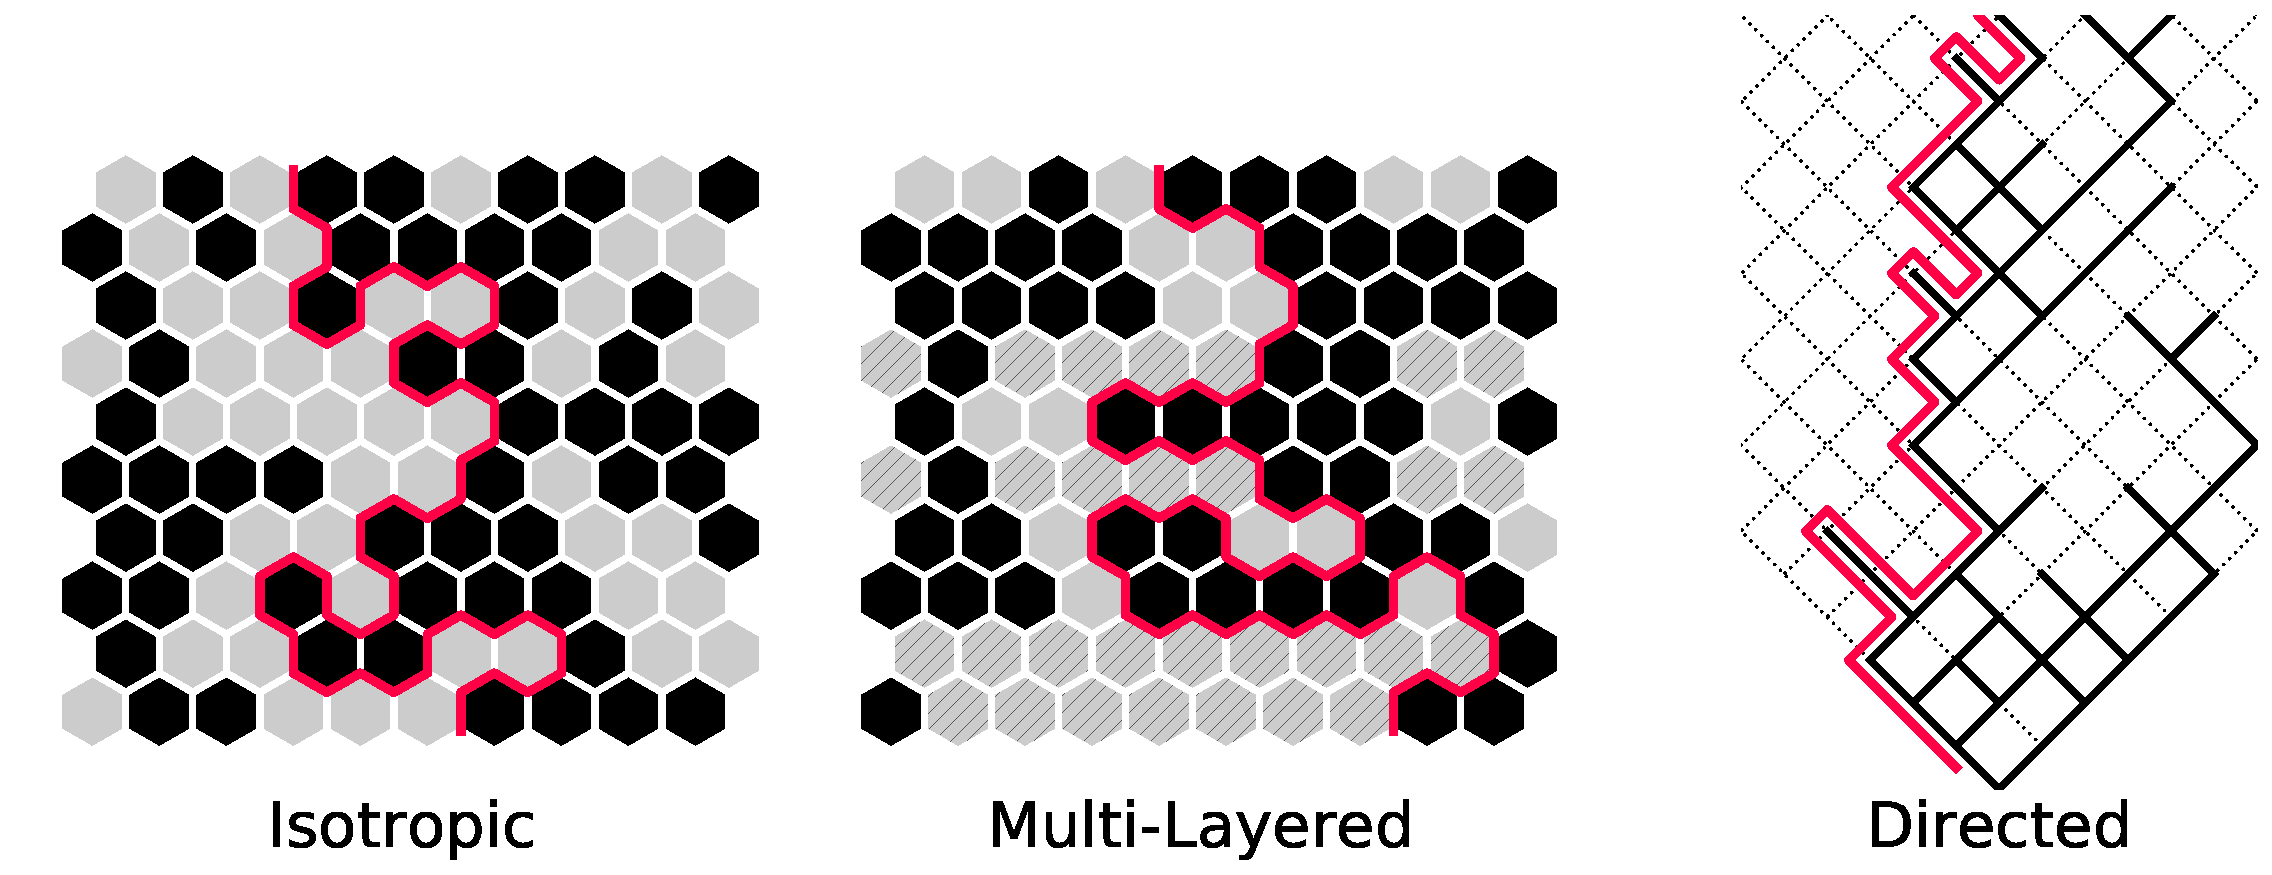
\includegraphics[width=0.8\textwidth]{chapters/ch6-asle/figs/models}
\end{center}
\caption{Percolation models used to generate the SLE curves. Isotropic
    percolation (left), where each site is occupied with the same probability
    $p$. Multi-layered percolation (middle), where some rows are occupied with
    probability $p+\Delta$ (dark gray rows) and others with $p-\Delta$ (light
    gray rows). Directed percolation (right) is a spreading process which
    starts at the bottom of the tilted lattice and can only advance upwards
    with probability $p$. The trace is defined as the perimeter of the
    percolating cluster.}
\label{fig:models}
\end{figure}

In this work we explore the possibility of using Loewner evolutions to study
anisotropic fractal systems, i.e., systems with different critical exponents in
each direction. These systems are not scale invariant, therefore not
conformally invariant either. We are particularly interested in the two
variants of the percolation model that show anisotropic behavior presented in
Sections~\ref{sec:mlp} and~\ref{sec:dp}, namely, multi-layered percolation and
directed percolation. Precisely, we generate the border of percolating
clusters (see Figure~\ref{fig:models}), numerically compute their corresponding
driving function, and then analyze the diffusive properties of these numerical
sequences. In the general case, we expect that the mean square displacement of
$U_t$ behaves like,
\begin{equation}
    \label{eq:diff}
    \left\langle U_t^2 \right\rangle \rightarrow b t^\alpha
\end{equation} 
as $t\rightarrow\infty$. In the case of traditional SLE, $\alpha=1$ and
$b=\kappa$.  The driving functions of anisotropic percolation models, we found,
display very distinctive anomalous diffusive behavior ($\alpha\neq1$). We also
look at the presence of long range correlations in the driving function using
the detrended fluctuation analysis (DFA). Finally, we show that our approach is
also valid in the opposite direction, that SLE consistently leads
anomalously diffusive driving functions to traces that display clear
anisotropic scaling. To test that, we generate Loewner traces driven by
fractional Brownian motions with different values of $b$ and $H=\alpha/2$,
which we will refer as $SLE(b,H)$, and compare the scaling properties of the
traces obtained with those of the lattice models.

\section{Methods}
\label{sec:methods}

Before delving into our results, we shall give a brief overview of some of the
most important methods used in the simulation and analysis of both traces
and driving functions.

\subsection{Generating Large Percolation Traces}
\label{sec:hulls}

Simulating the percolation process and extracting the percolating cluster
perimeter is very straightforward and a number of good algorithms are
available. However, because of the spotty behavior of the zipper algorithm (see
Fig.~\ref{fig:eulerzip}) in the high $\kappa$ ($>4$) domain, we need very large
traces in order to obtain reliable results. The usual algorithms are normally
very memory hungry because you need to store the state of all sites of the
lattice. Since we are only interested in obtaining the perimeter of the
percolating cluster, which consists of only a small portion of the lattice, one
might imagine if there is a more efficient way of simulating these curves.
Luckily there is, thanks to the locality property of the percolation model. The
method is called the \textit{percolation exploration process}~\cite{Cardy2005}.

\begin{figure}[b]
\begin{center}
    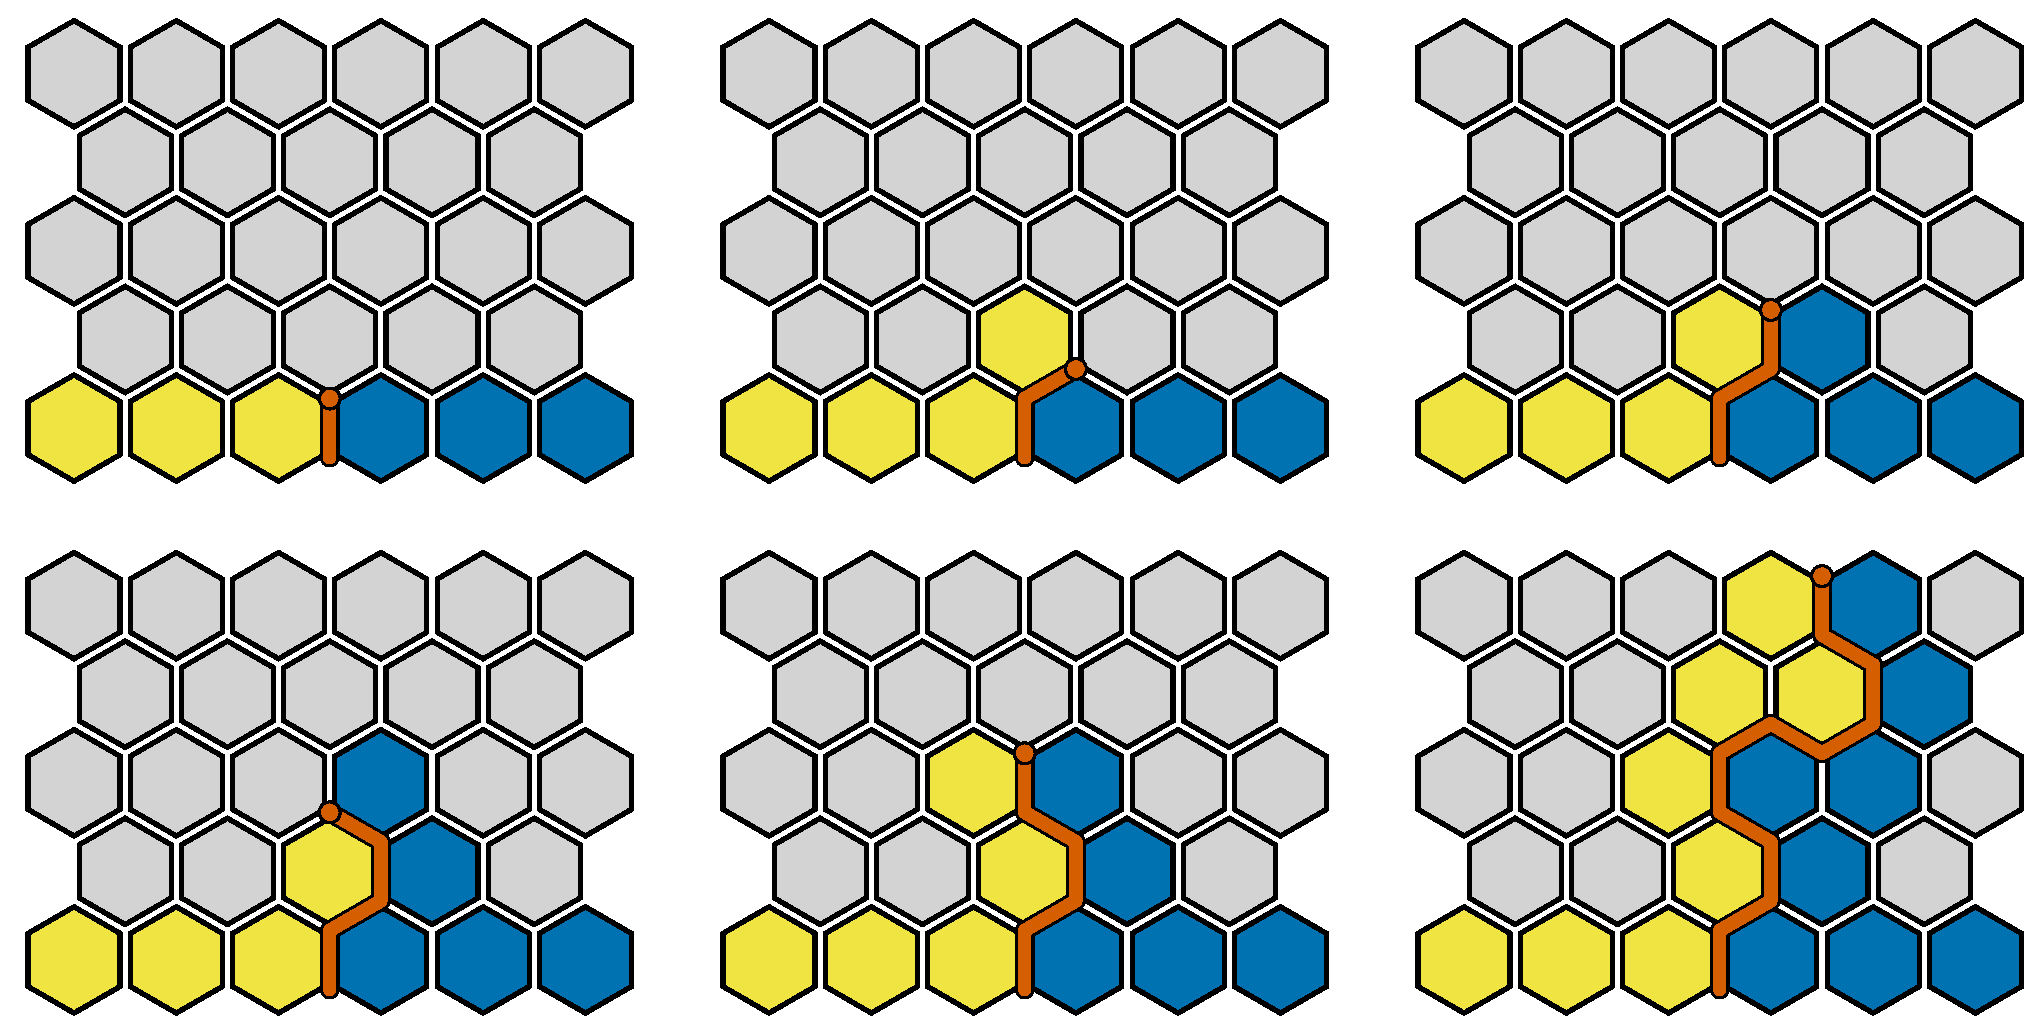
\includegraphics[width=0.8\textwidth]{chapters/ch6-asle/figs/explore}
\end{center}
\caption{The first few steps of a percolation exploration process with closed
    boundary conditions in a triangular lattice, which means the left side of
    the bottom row is always unoccupied (yellow) and the right side is always
    occupied (blue). At each step, the walker checks the status of the site
    right in front of it. If it is yellow, the walker turns clockwise and takes
    a step. If it is blue it turns counter-clockwise before taking a step. This
    method is superior because you only need to store the information about the
    sites adjacent to the curve, saving RAM and allowing for simulations of
    very large traces.}
\label{fig:explore}
\end{figure}


The exploration process is easier to define in the triangular lattice, because
at any given time the walker is always facing a single site, unlike the square
lattice, in which it faces two sites at once, complicating things a little (it
does not make it impossible, though). In the exploration process, a walker is
put in an initial position at the bottom of the lattice. The walker observes
the state of the site right in front of him. If it is unoccupied, the walker
turns clockwise, otherwise it turns clockwise. Then the walker takes a step in
the direction it is facing. This process is then repeated until one obtain a
curve long enough. The algorithm guarantees that the curve will not
self-intersect and will not get trapped.

Because we restrict ourselves to chordal SLE, the walker can never leave the
upper-half plane. To assure this, we impose closed boundary conditions in which
the left side of the bottom row of the lattice is always unoccupied and the
right side is always occupied. This way the trace will always turn away from
the real line.

It is pretty clear the advantage of this method, you only need to store the
information about the sites directly adjacent to the perimeter, which can be
cached in your container of preference, like a hash table (also known as maps
or dictionaries), as illustrated in Figure~\ref{fig:explore}. This allow us to
simulate traces with up to million points. In fact we could easily go above
that, the limiting factor being the time the zipper algorithm takes to compute
the driving function.

\begin{figure}[t]
\begin{center}
    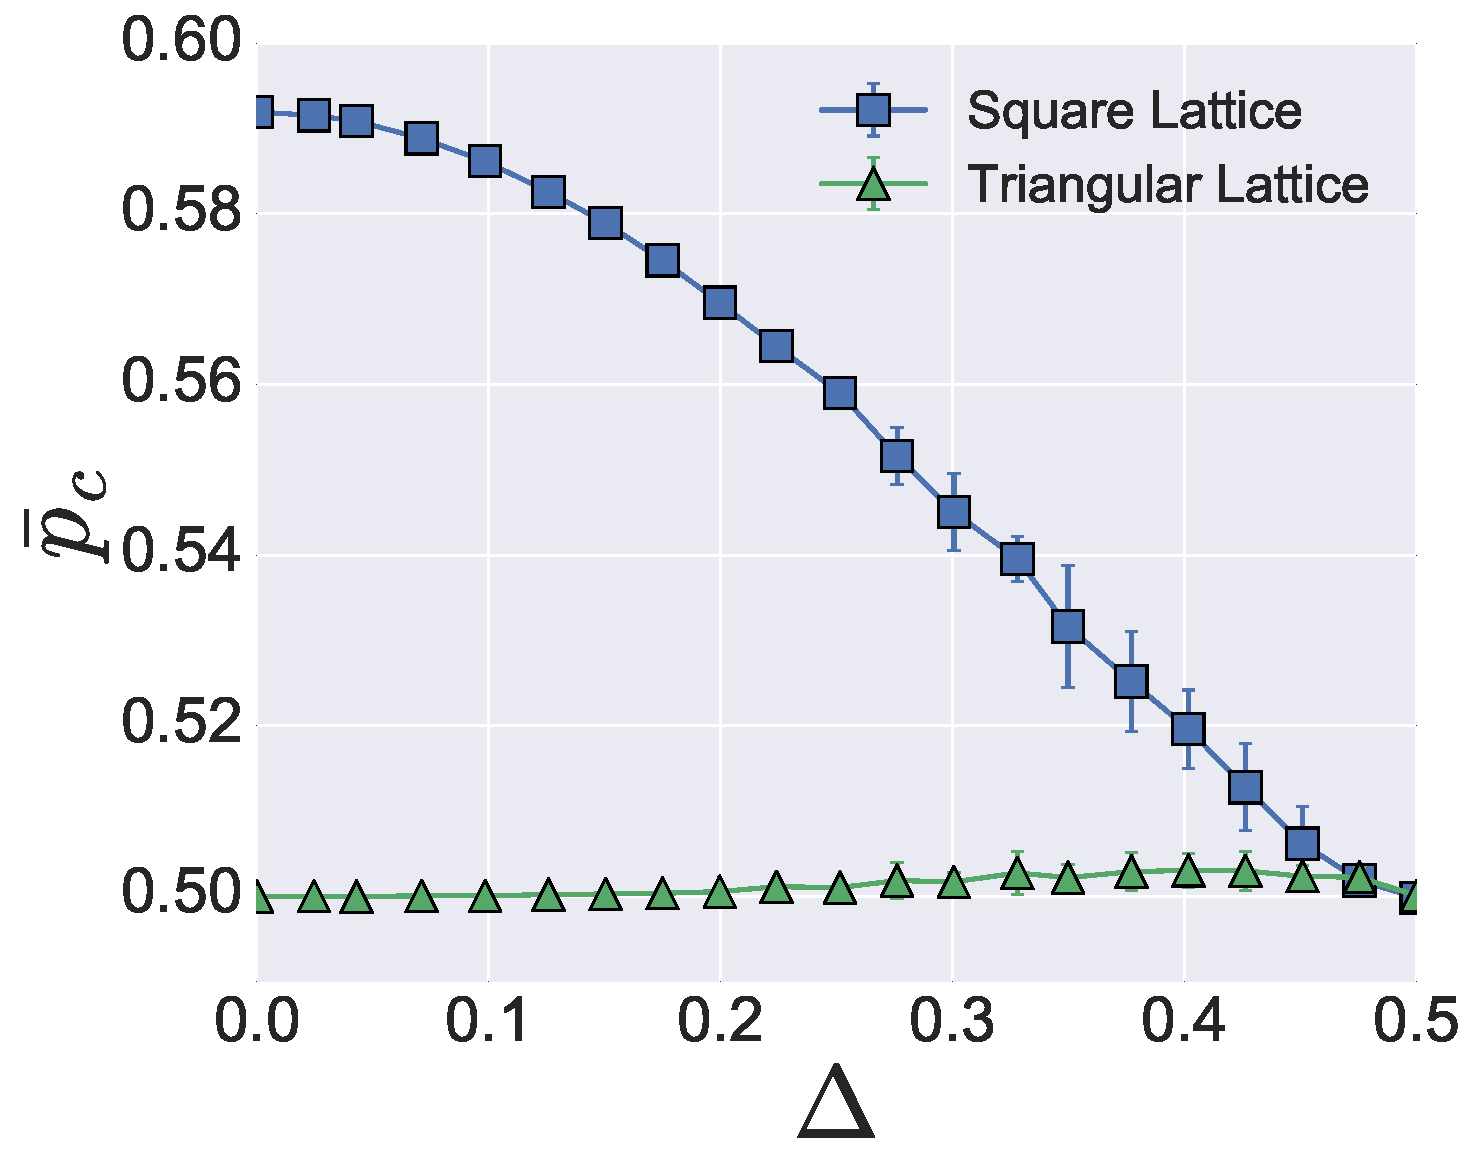
\includegraphics[width=0.6\textwidth]{chapters/ch6-asle/figs/mlp_ps}
\end{center}
\caption{Critical point of multi-layered percolation as computed using the
    cluster perimeter method. This is done by generating several percolation
    perimeters without boundary conditions until they form a loop. In the
    critical point the loop has equal probabilities of being a internal or
    external perimeter. We found that in the triangular lattice, $p_c=0.5$
    for every value of $\Delta$, unlike the square lattice.}
\label{fig:mlp_ps}
\end{figure}

We used the exploration process to generate the traces for isotropic and
multi-layered percolation in a triangular lattice. However, the critical point
of multi-layered percolation have not yet been determined in the triangular
lattice. To compute $p_c(\Delta)$ we made use the cluster perimeter
method~\cite{Ziff1986}. We basically use the exploration process with no
boundary condition to generate curves until they form a loop. If the loop is
formed clockwise, this means it represents the perimeter of a hole inside a
cluster. If it is counterclockwise, it means the curve is the outside perimeter
of cluster. On the critical point, the probability that a loop is internal or
external is the same. We found, somewhat surprisingly, that in the triangular
lattice, $p_c=0.5$ for every value of $\Delta$, unlike the square lattice, as
shown in Figure~\ref{fig:mlp_ps}.

This algorithm is not appropriate for the simulation of directed percolation
traces, because the occupation probability of any given site is not independent
from its neighbors. In this case we decided for a more standard approach,
growing a cluster using a graph data structure to save memory, and finding the
perimeter using a simple walker algorithm, where the trace is the trajectory of
a particle that moves along the border of the cluster while keeping the cluster
always at to right hand side.

\subsection{Detrended Fluctuation Analysis}
\label{sec:dfa}

We want to test whether or not the driving functions present long range
correlations. Other works have shown that some form of anisotropy can be
observed in SLE traces driven by L\'evy processes. We have good reasons to
believe this is not the case for multi-layered and directed percolation,
because L\'evy processes do not show subdiffusion and they generate
discontinuous traces.

In order to close the issue we perform one last test: check for the presence of
long range correlations. To do that we employ a method called Detrended
Fluctuation Analysis (DFA), which is an adaptation of an older
algorithm called simply fluctuation analysis. It is specially designed for the
analysis of non stationary series~\cite{Peng1993, Hardstone2012} with the
objective of computing their Hurst exponent $H$. This quantity measure the
presence of long term correlations, and is found in the interval $H\in[0,1]$,
where $H=0.5$ means that the series has no long range correlations. The case
$H<0.5$ means the series is anti-persistent, so fluctuations in one direction
tend be followed by fluctuations in the opposite direction. When $H>0.5$, the
series is persistent~\cite{Matos2008} and fluctuations tend to happen in the
same direction.

Given a time series of $N$ data points $\{x_i\}$, we first generate a random walk
out of it by making the cumulative profile of the series
\begin{equation}
    X_i = \sum_{i=1}^{N} \left({x_i - \left\langle x \right\rangle}\right).
\end{equation}
The accumulated series is then divided in $m$ non overlapping partitions, each with
$s = N/m$ elements. In case $N$ is not divisible by $m$ we can still make use
of the last elements of the series by taking $s=\left\lfloor N/m\right\rfloor$
and reflecting it in the end the following way
\begin{equation}
    X\rightarrow\left\{X_1, \ldots, X_{ms},
                       X_{N}, X_{N - 1}, \ldots,
                       X_{N - ms}\right\}.
\end{equation}
In this case we actually changed the series size to $N\rightarrow2ms$ and the
number of intervals to $m\rightarrow2m$, so this should be taken in account in
later equations. This step is optional, but useful in order to use all the
information embedded in the time series.

\begin{figure}
    \begin{center}
        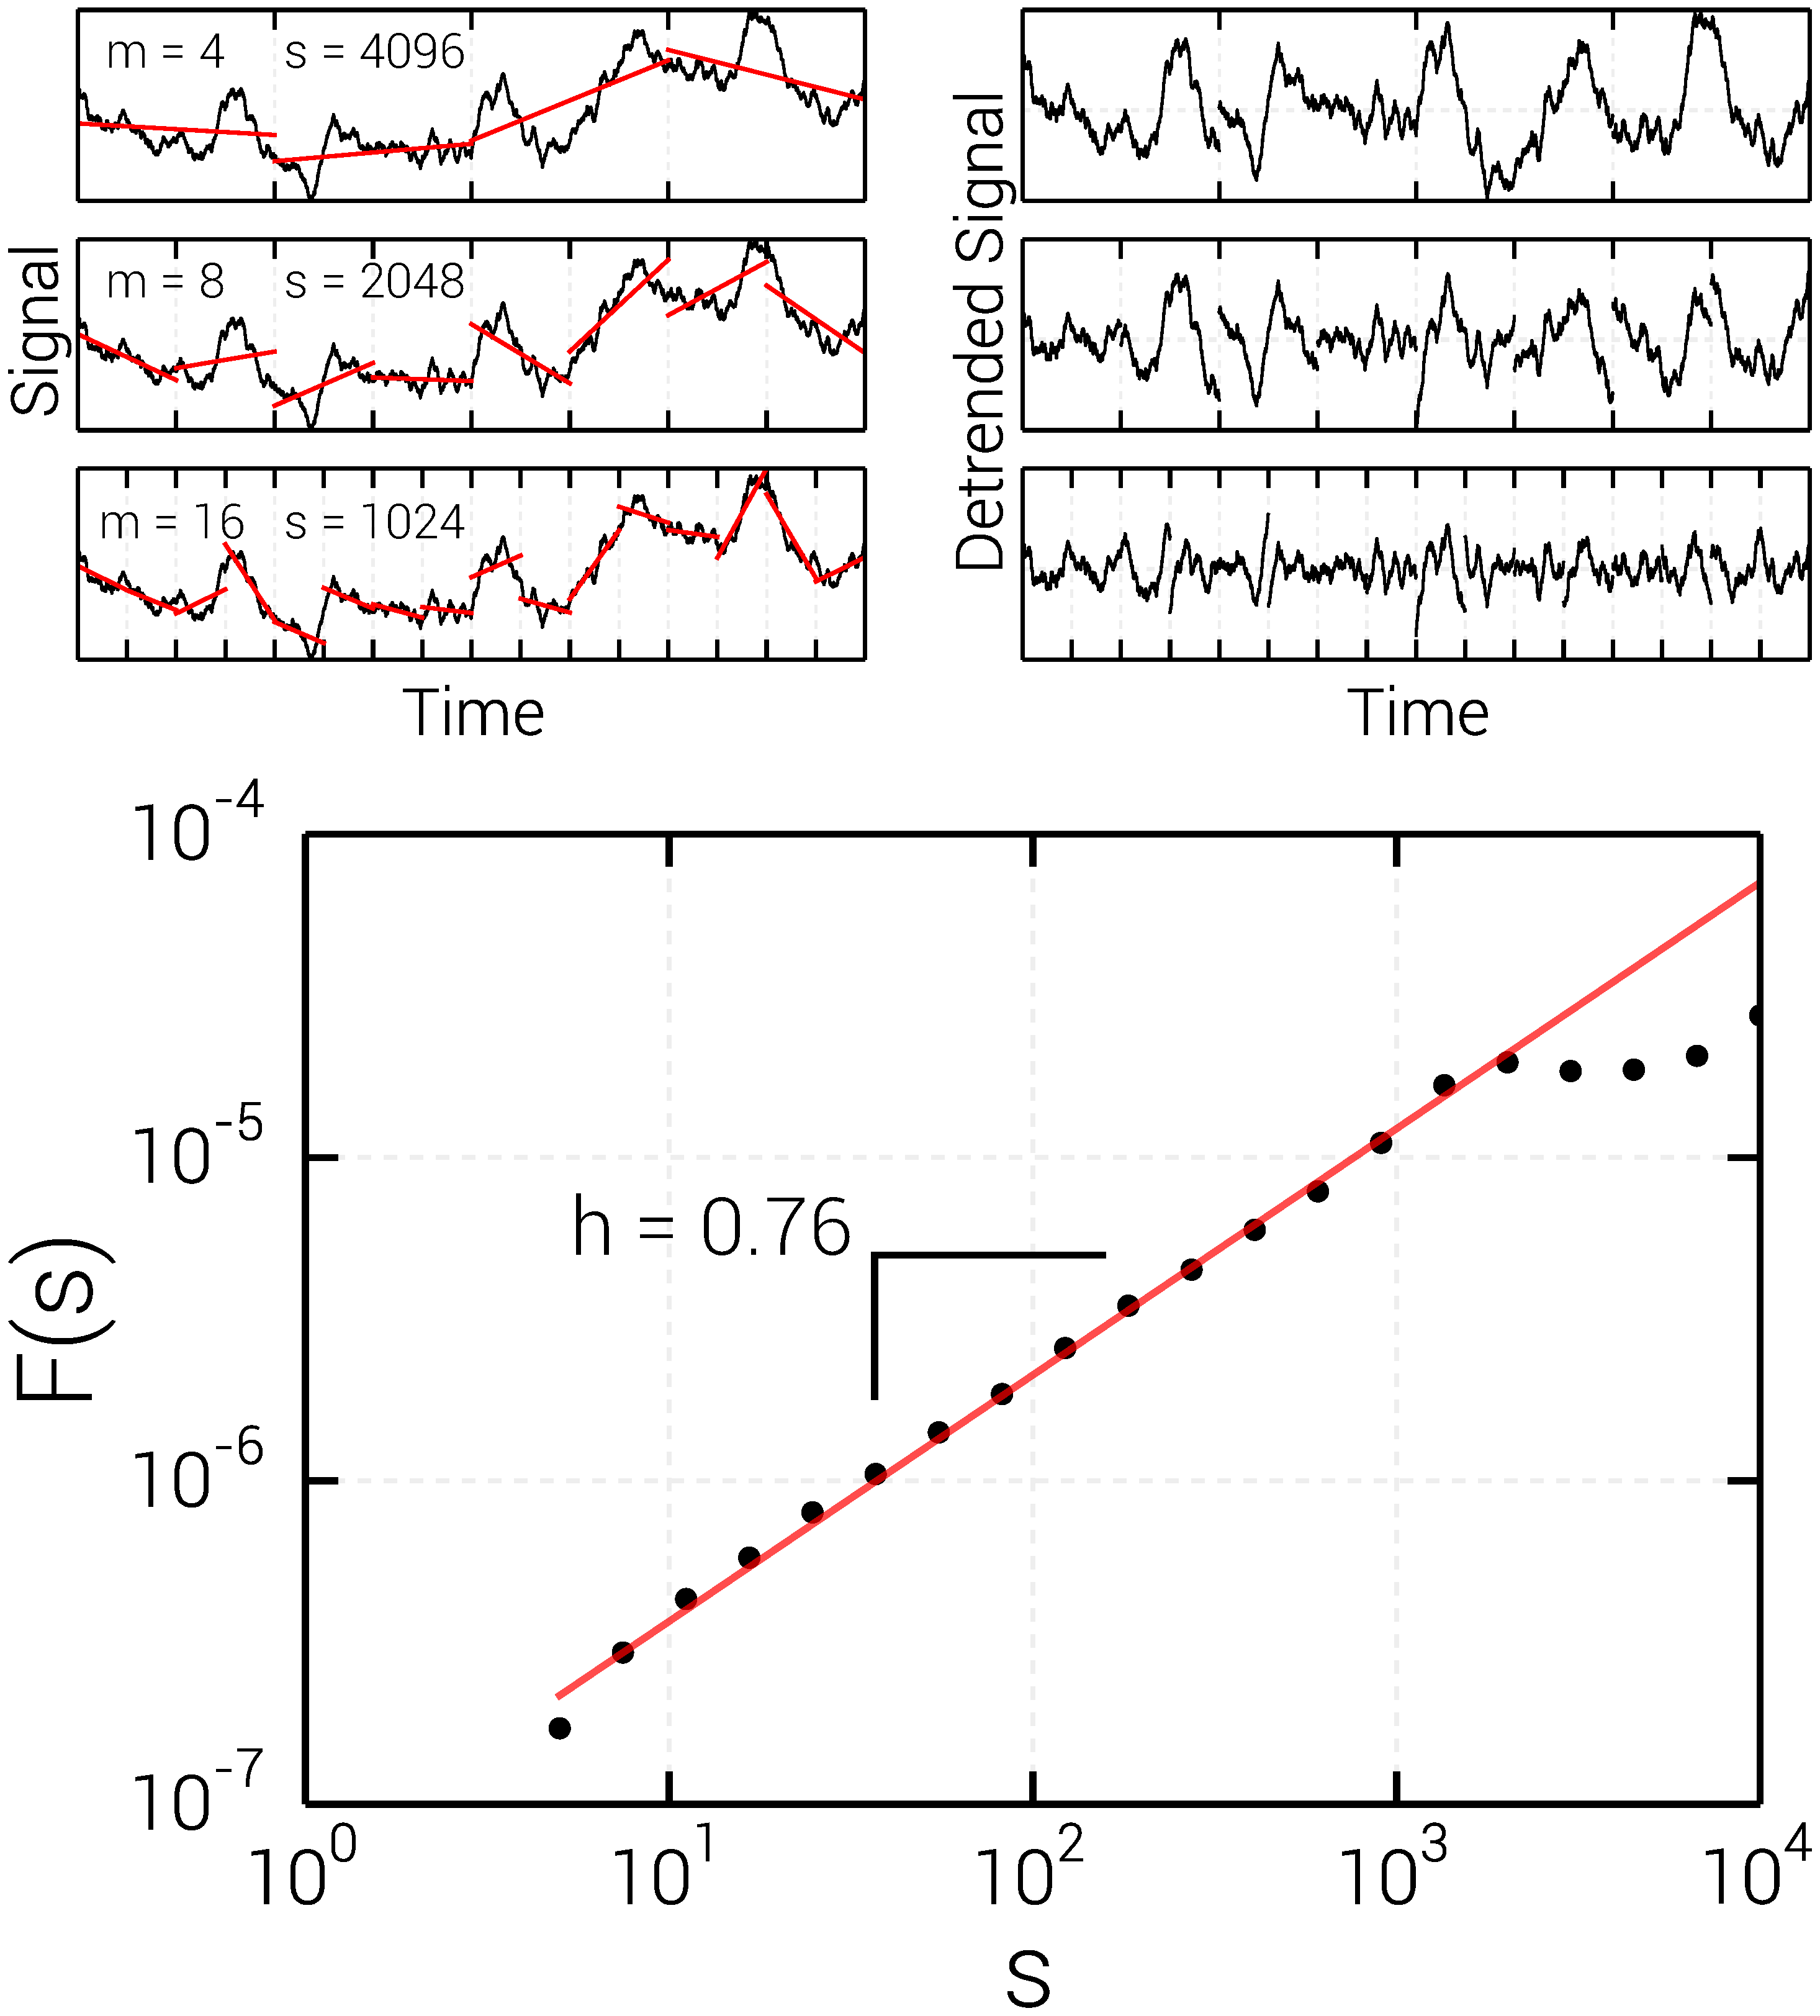
\includegraphics[width=0.6\textwidth]{chapters/ch6-asle/figs/dfa}
    \end{center}
    \caption{The Detrended Fluctuation Analysis (DFA) of a time series of
        $N=16,384$ data points. First we divided the series in $m$ partitions with
        $s$ points each (top-left), then fitted each separately with a first order
        polynomial $f_1(i)$ (red lines), obtaining the detrended series by subtracting
        the signal by the trend (top-right).  The fluctuation function (the standard
        deviation of the detrended signal) is computed for various values of $s$
        (bottom).  The Hurst exponent is then determined by fitting the fluctuation
        function with a power law $F(s)\sim s^h$.}
\label{fig:dfa}
\end{figure}

We then determined the trend of each partition by fitting them separately using
a polynomial of degree $v$. Usually a first or second degree polynomial is
chosen. The series is detrended by taking the difference of the signal value and
the trend 
\begin{equation}
    Y_i = \sum_{i=1}^{N} X_i - f_v(i),
\end{equation}
where $f_v(i)$ is the value of the trend in the point $i$. We define the fluctuation
function as the standard deviation of the detrended signal, which is a function
of the number of points $s$ in each partition of the time series
\begin{equation}
    F(s) = \sqrt{\frac{1}{N}\sum_{i=1}^{N}Y_i}.
\end{equation}

A plot of $F(s)$ vs. $s$ in a log-log scale should show a straight line for
well a behaved series (see Fig.~\ref{fig:dfa}). The Hurst exponent of the
series can be determined by fitting the fluctuation function with a power law
\begin{equation}
    F(s)\sim s^H.
\end{equation}

\subsection{Generating Fractional Brownian Motions}
\label{sec:fbm}

We want to generate fractional Brownian motions $B_t$ such that
\begin{equation}
    \label{eq:fbm}
    \left\langle B_t^2 \right\rangle = bt^{2H}.
\end{equation}
There are several methods to generate this process numerically, but not all of
them give you ample control over the prefactor $b$, although most are very
accurate in $H$. A method that adequately fulfills this criterion is the
Davies-Harte algorithm~\cite{Davies1987}. It can be used to generate any
stationary Gaussian process for which the autocovariance sequence is known. In
the case of the fractional Brownian motion, it takes the form
\begin{equation}
    c_i = \frac{b}{2} \left(
            \left|i+1\right|^{2H} +
            \left|i-1\right|^{2H} -
            2\left|i\right|^{2H}
          \right)
\end{equation}

To obtain a series of length $N$ we generate the following sequence of $2N$
points
\begin{equation}
    s_i=\left\{c_{0},c_{1},\ldots,c_{N},c_{N-1},\ldots,c_{1}\right\}
\end{equation}
and compute its discrete Fourier transform, that is
\begin{equation}
    g_{i}=\sum_{j}s_{j}e^{-i\pi kj/N}.
\end{equation}
This operation can be done in $O(N\log N)$ operations using a fast Fourier
transform~\cite{Frigo2002}. The $g_i$ are real valued, but a necessary condition for the
Davies-Harte algorithm to work is that they also be nonnegative. It is
important to check for this condition even if just for debugging purposes,
as it catches a lot of small mistakes.

Let $W_{i\in[0,N]}$ be a sequence of $N+1$ random complex numbers where the
real and imaginary parts are independently distributed according to a normal
distribution with zero mean and unit variance. We then construct the series
\begin{equation}
    Y_{i\in[0,2N-1]}=\begin{cases}
        \sqrt{2Ng_{i}}\mbox{Re}\left\{ W_{i}\right\}  & \mbox{if } i=0,N\\
        \sqrt{Ng_{i}}W_{i} & \mbox{if } i\in\left[1, N-1\right]\\
        \sqrt{Ng_{i}}W_{2N-i}^{*} & \mbox{if } i\in\left[N+1, 2N-1\right]
    \end{cases},
\end{equation}
where $W^{*}$ is the complex conjugate. The fractional Brownian motion $B_t$ is
obtained by computing the inverse Fourier transform of this series. Although
the obtained series have $2N$ points we discard the second half, as it is not
guaranteed to be well behaved. The $B_t$ are defined for $t\in{0,1,\ldots,N-1}$,
but the series can easily be rescaled for any timespan desirable by applying
the relation
\begin{equation}
    B_{t\in[0,t_{f}]}={\left(\frac{t_{f}}{N}\right)}^{H}B_{t\in[0,N]}.
\end{equation}

In Figure~\ref{fig:fbm}, we show some examples of fractional Brownian motion
generated using this algorithm. We also show that the mean squared displacement
behaves as described by Eq.~\ref{eq:fbm}.

\begin{figure}
\begin{center}
    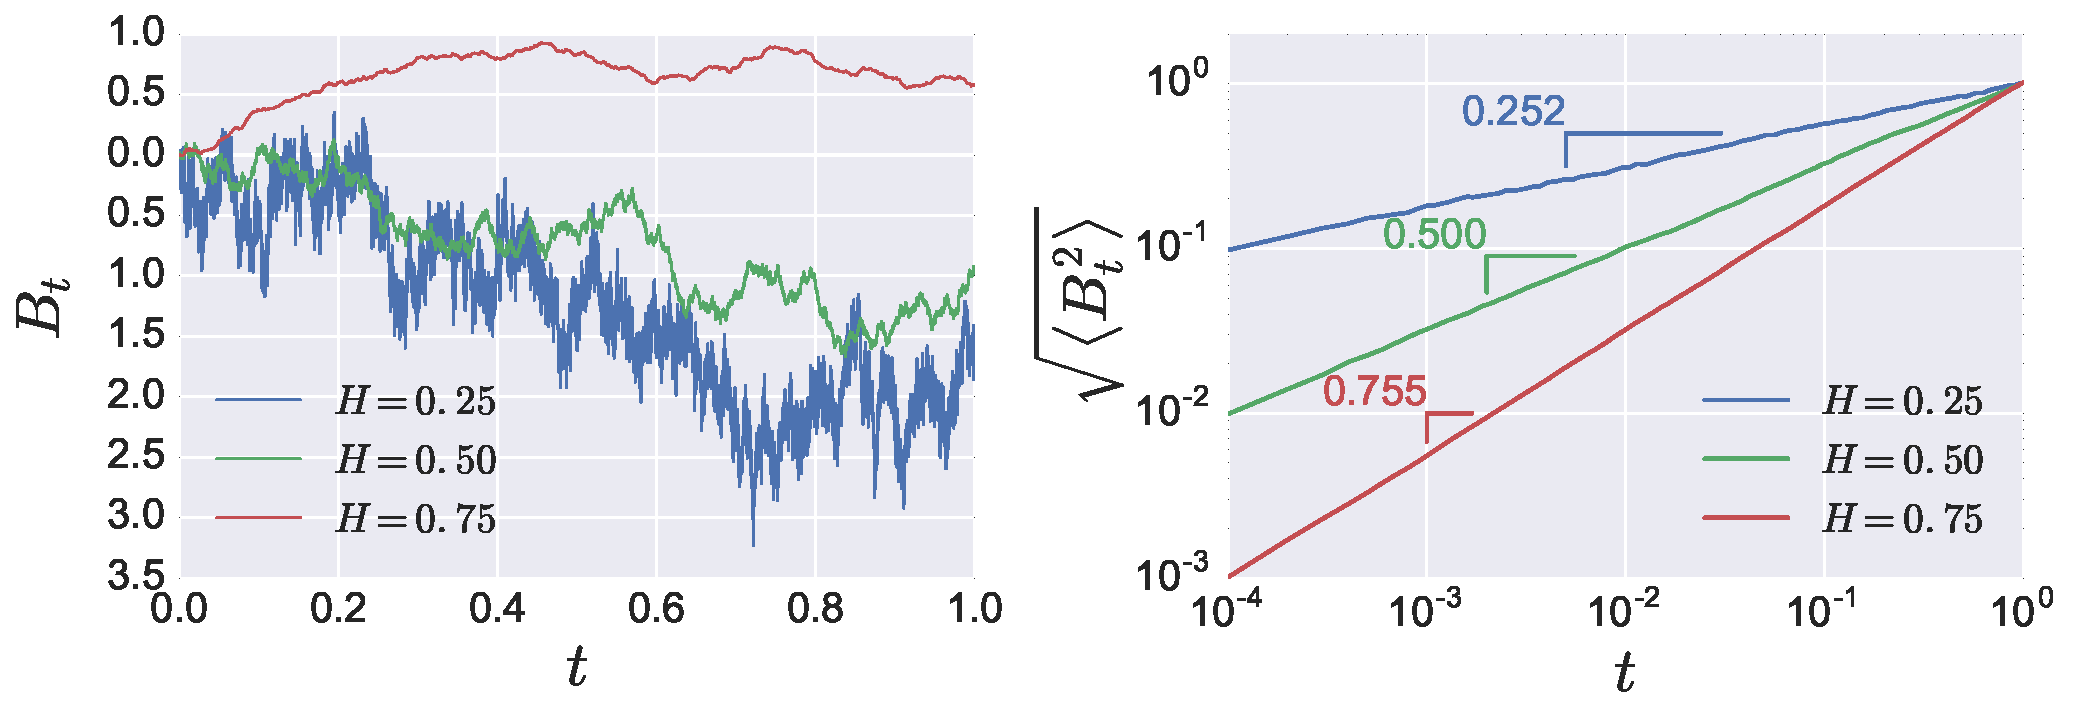
\includegraphics[scale=0.45]{chapters/ch6-asle/figs/fbm}
\end{center}
\caption{Example of three fractional Brownian motions generated using the
    Davies-Harte algorithm (left). They all have $b=1.0$ and different values
    of $H$. We also show the behavior of the mean square displacement of the
    scaling properties of the curves. We found that the mean square displacement
    scales as $\sqrt{\left\langle B_t^2\right\rangle}=\sqrt{b}t^H$ with
    parameters very similar to the input given.}
\label{fig:fbm}
\end{figure}


\section{Results and Discussion}
\label{sec:scaling}

\begin{figure}
\begin{center}
    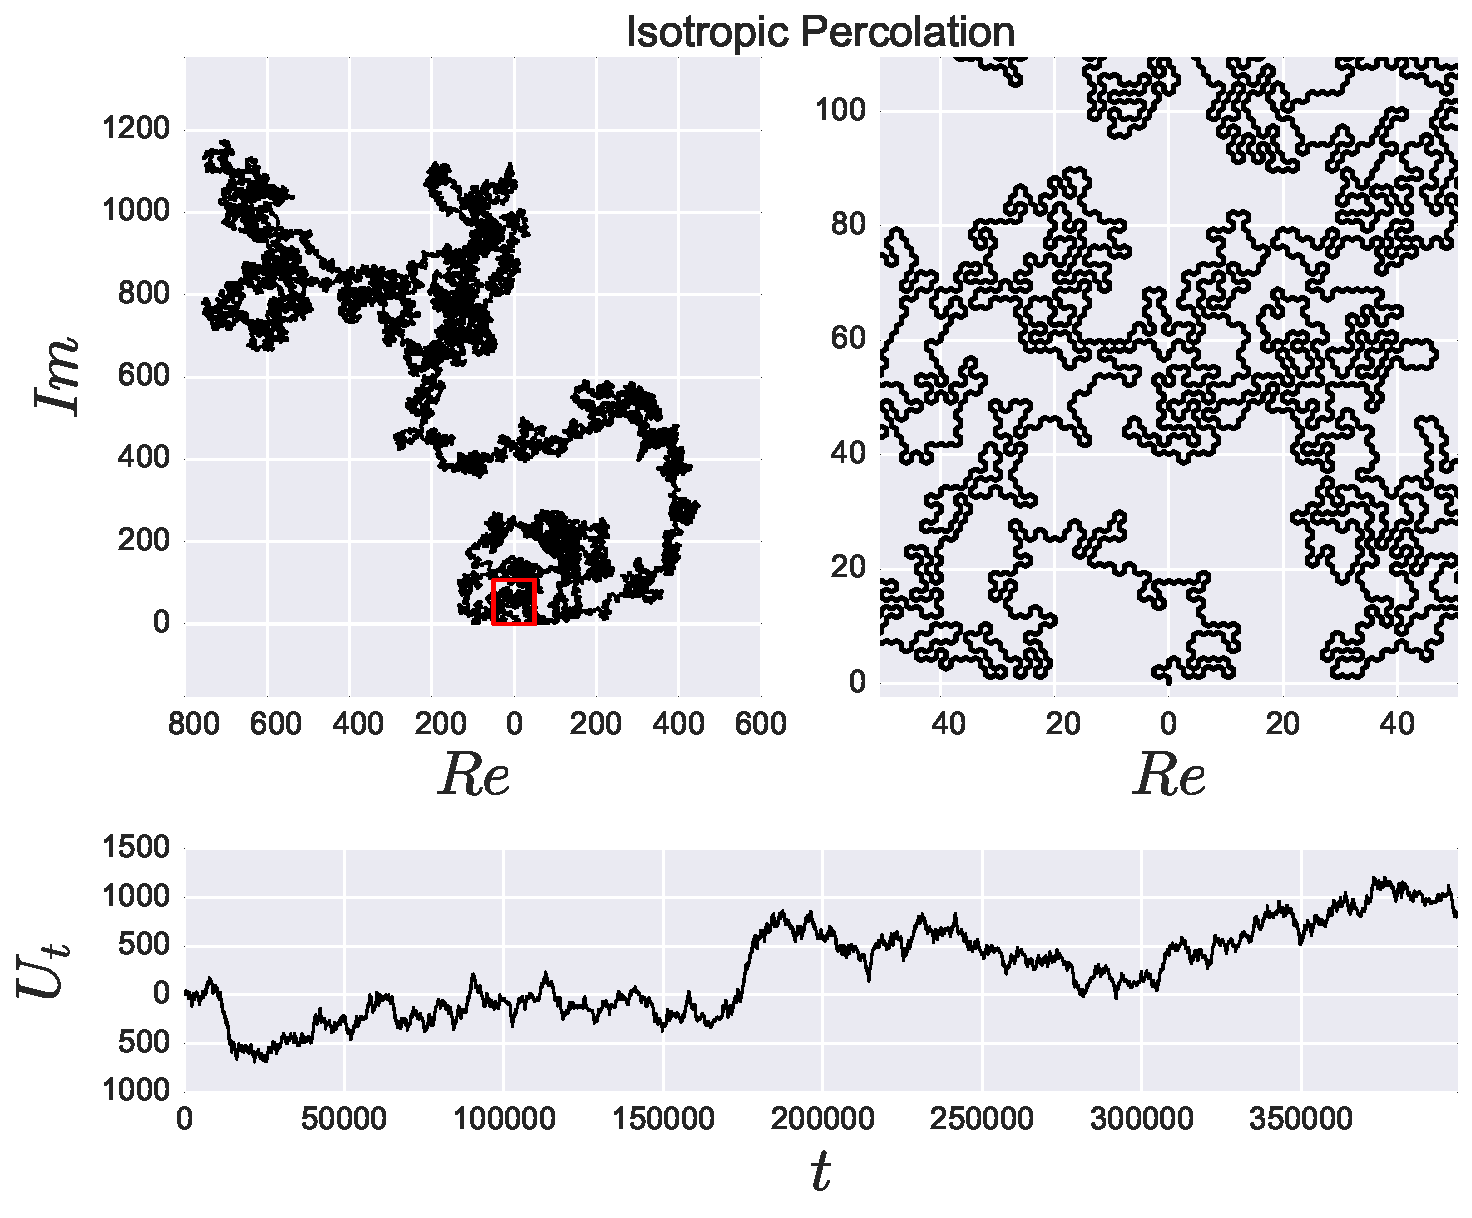
\includegraphics[width=0.65\textwidth]{chapters/ch6-asle/figs/ip_trdr}
\end{center}
\caption{Example of a cluster perimeter of the isotropic percolation model in
    the triangular lattice with a detail shown. The bottom graph is the driving
    function obtained by applying the zipper algorithm to this trace.}
\label{fig:ip_trdr}
%\end{figure}

%\begin{figure}
\begin{center}
    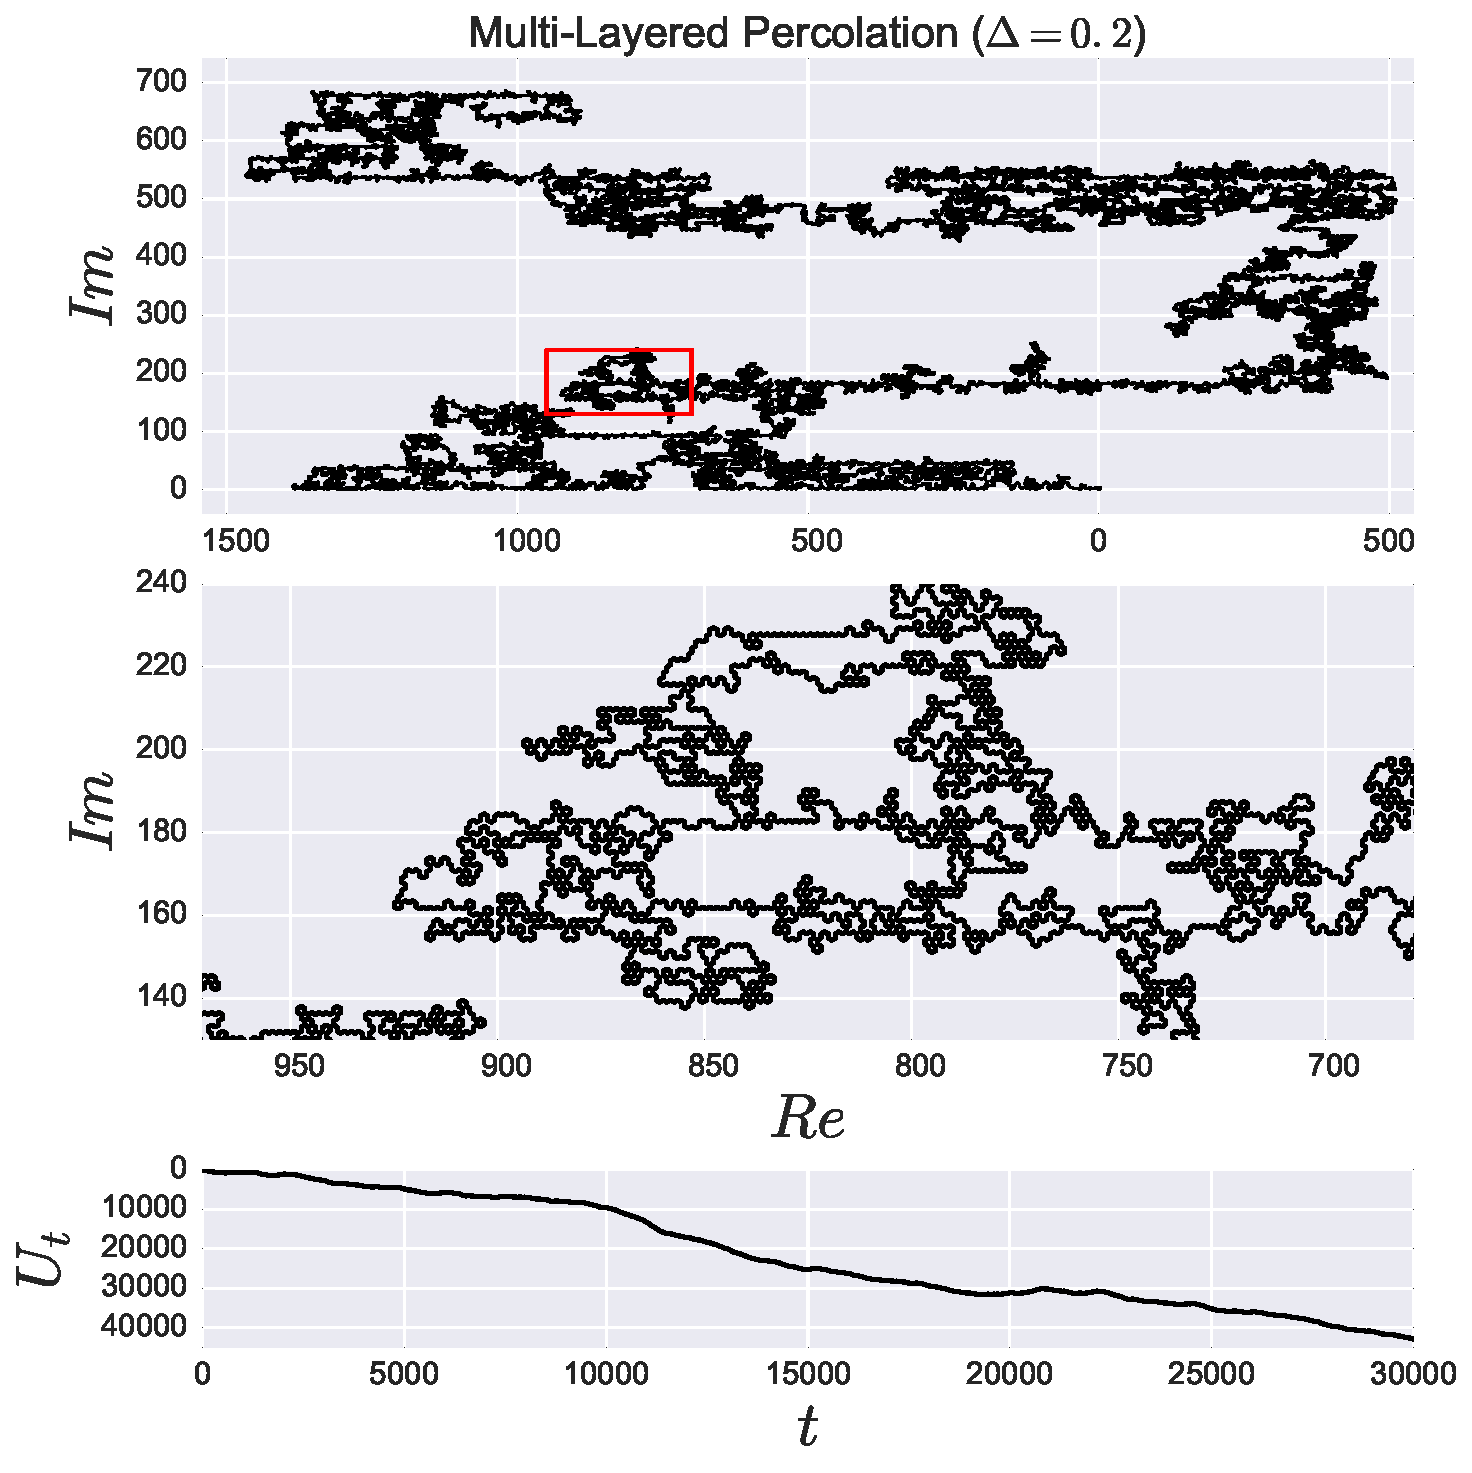
\includegraphics[width=0.65\textwidth]{chapters/ch6-asle/figs/ml_trdr}
\end{center}
\caption{Example of a cluster perimeter of the multi-layered percolation model
    in the triangular lattice ($\Delta=0.2$) with a detail shown. The bottom
    graph is the driving function obtained by applying the zipper algorithm to
    this trace.}
\label{fig:ml_trdr}
\end{figure}

\begin{figure}
\begin{center}
    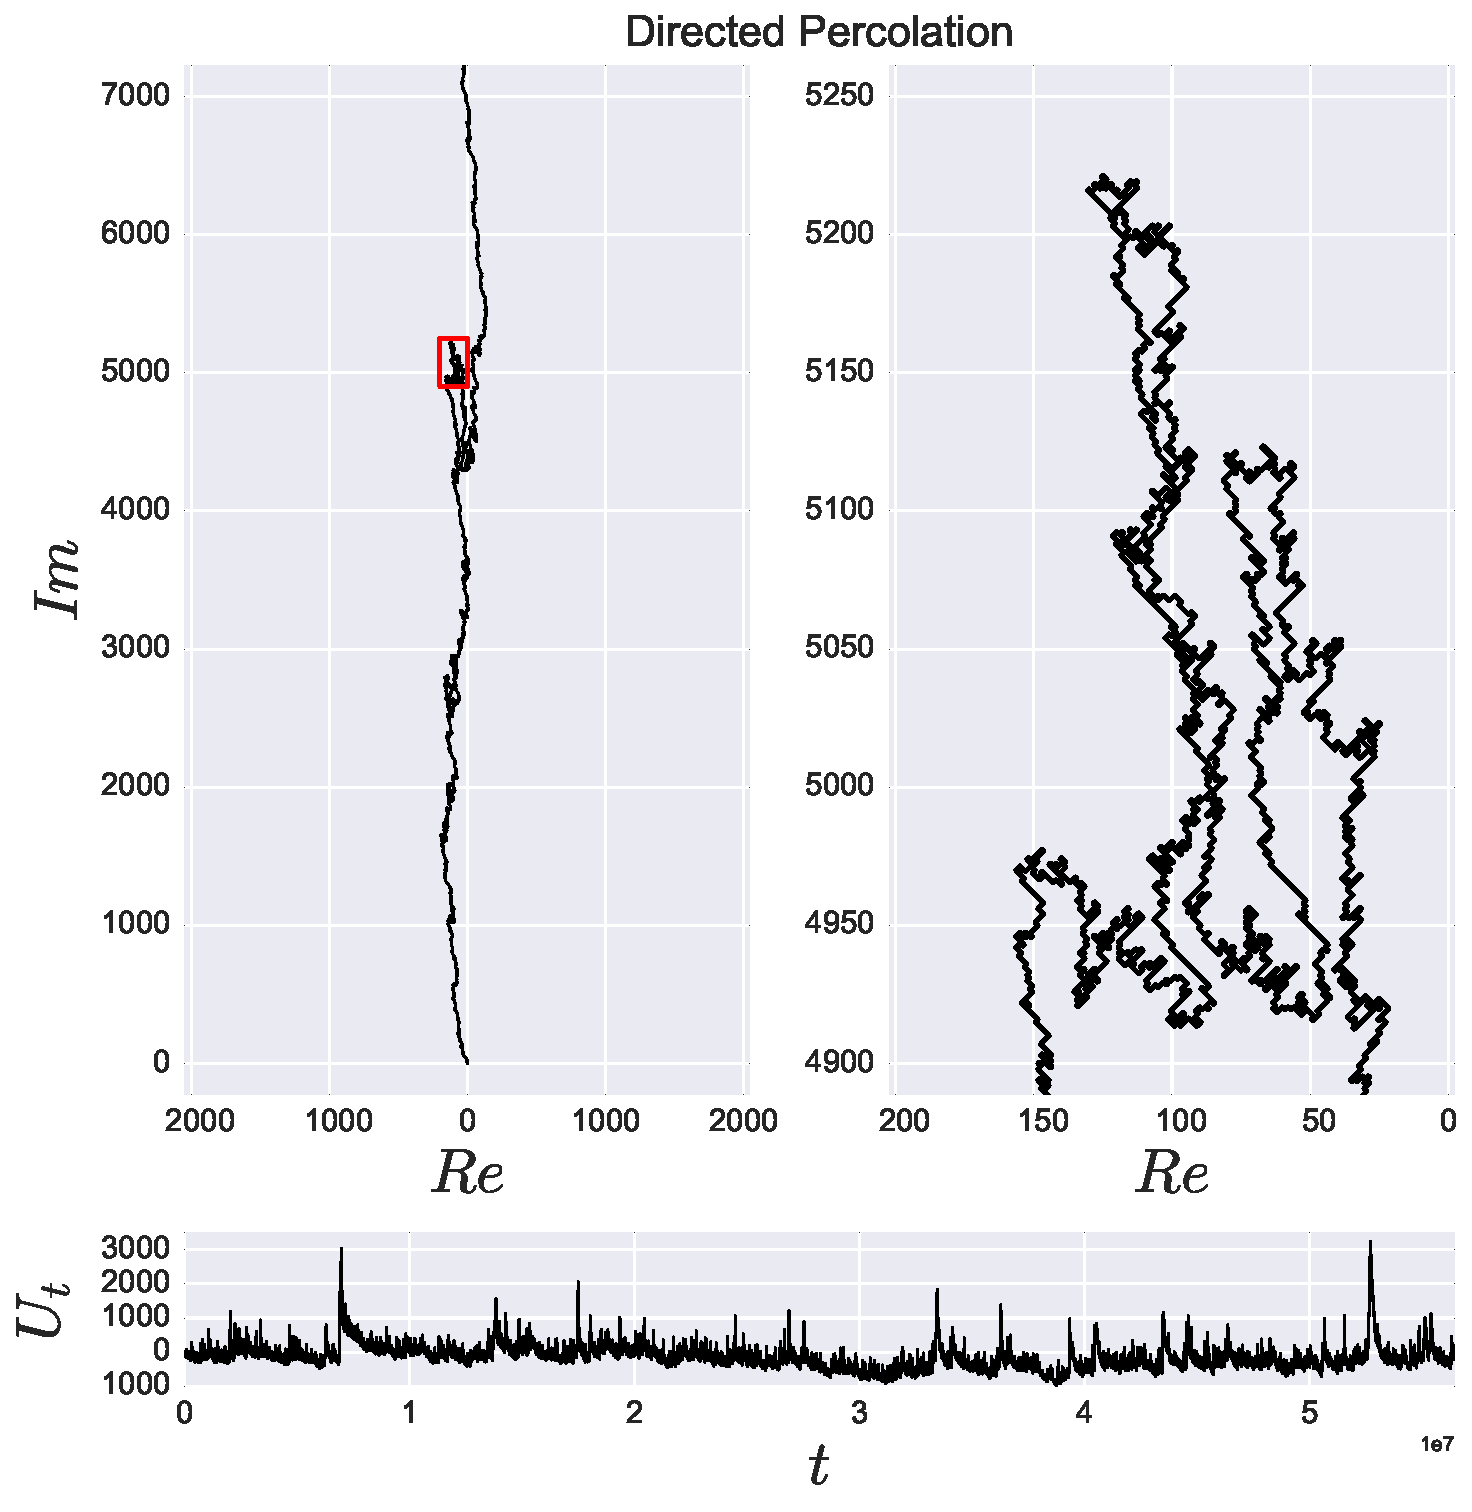
\includegraphics[width=0.65\textwidth]{chapters/ch6-asle/figs/dp_trdr}
\end{center}
\caption{Example of a cluster perimeter of the bond directed percolation model
    in the square lattice with a detail shown. The bottom graph is the driving
    function obtained by applying the zipper algorithm to this trace.}
\label{fig:dp_trdr}
\end{figure}

As mentioned, we set up to study the properties of the driving functions of
traces generated by multi-layered and directed percolation. As a control for
our tests we also analyzed isotropic percolation, which is well understood
theoretically.

We generated an ensemble of $10^4$ cluster perimeters for each model at
criticality. Isotropic and multi-layered curves were generated on a triangular
lattice, while the directed percolation ones were done in a square lattice. The
traces had a length of $10^5$ lattice units. Using the zipper algorithm
described in Section~\ref{ss:zipper}, we computed the driving function of each
curve. The output of the algorithm is a sequence of time instants and their
respective value of the drive, $\{(t_0=0, U_{t_0}=0), (t_1, U_{t_1}), \ldots,
(t_N, U_{t_N})\}$. This algorithm, however, does not guarantee that the
discretized times $t_i$ are equally spaced, even for curves of same length and
step size. To facilitate further analysis, we create a new sequence
$\{(\tilde{t}_{0}, U_{\tilde{t}_{0}}), (\tilde{t}_{1}, U_{\tilde{t}_{1}}),
\ldots, (\tilde{t}_{M}, U_{\tilde{t}_{M}})\}$, where $\tilde{t}_k = t_f^{k/M}$
and $U_{\tilde{t}_k}$ is computed through a linear interpolation of the
$U_{t_i}$. We used $M=20,000$ and the values of $t_f$ were different for each
model chosen as the smallest value of $t_N$ among all the samples. The exact
values can be found in Table~\ref{tab:param}.
Figures~\ref{fig:ip_trdr},~\ref{fig:ml_trdr}, and~\ref{fig:dp_trdr} show
examples of the kind of curves obtained as well as their computed driving
function.

\subsection{Diffusion analysis}
\label{sec:dif}

We can now analyze the diffusive properties of the driving function. We do this
by looking at the mean square displacement, that it, $\left\langle U_t^2
\right\rangle$, where $\left\langle\cdot\right\rangle$ is the mean over the
samples. As mentioned in Section~\ref{sec:levy}, we expect that
\begin{equation}
    \left\langle U_t^2 \right\rangle\sim bt^\alpha.
\end{equation}
In a log-log graph the means squared displacement should appear as a line, so
we can obtain the values of $b$ and $\alpha$ through an ordinary least square
fitting. Figure~\ref{fig:diffusion} show the results and the exact values of
$b$ and $\alpha$ obtained can be found in Table~\ref{tab:diff}. We observed the
expected behavior from the isotropic percolation with $\alpha\approx1.0$ and
$b\approx6.2\pm0.3$, which is coherent with the expected value of $b=\kappa=6$.
The large error bar is a result of the spotty behavior of the zipper algorithm
in the high ($>4$) $\kappa$~\cite{Kennedy2007}.

\begin{figure}[b]
\begin{center}
    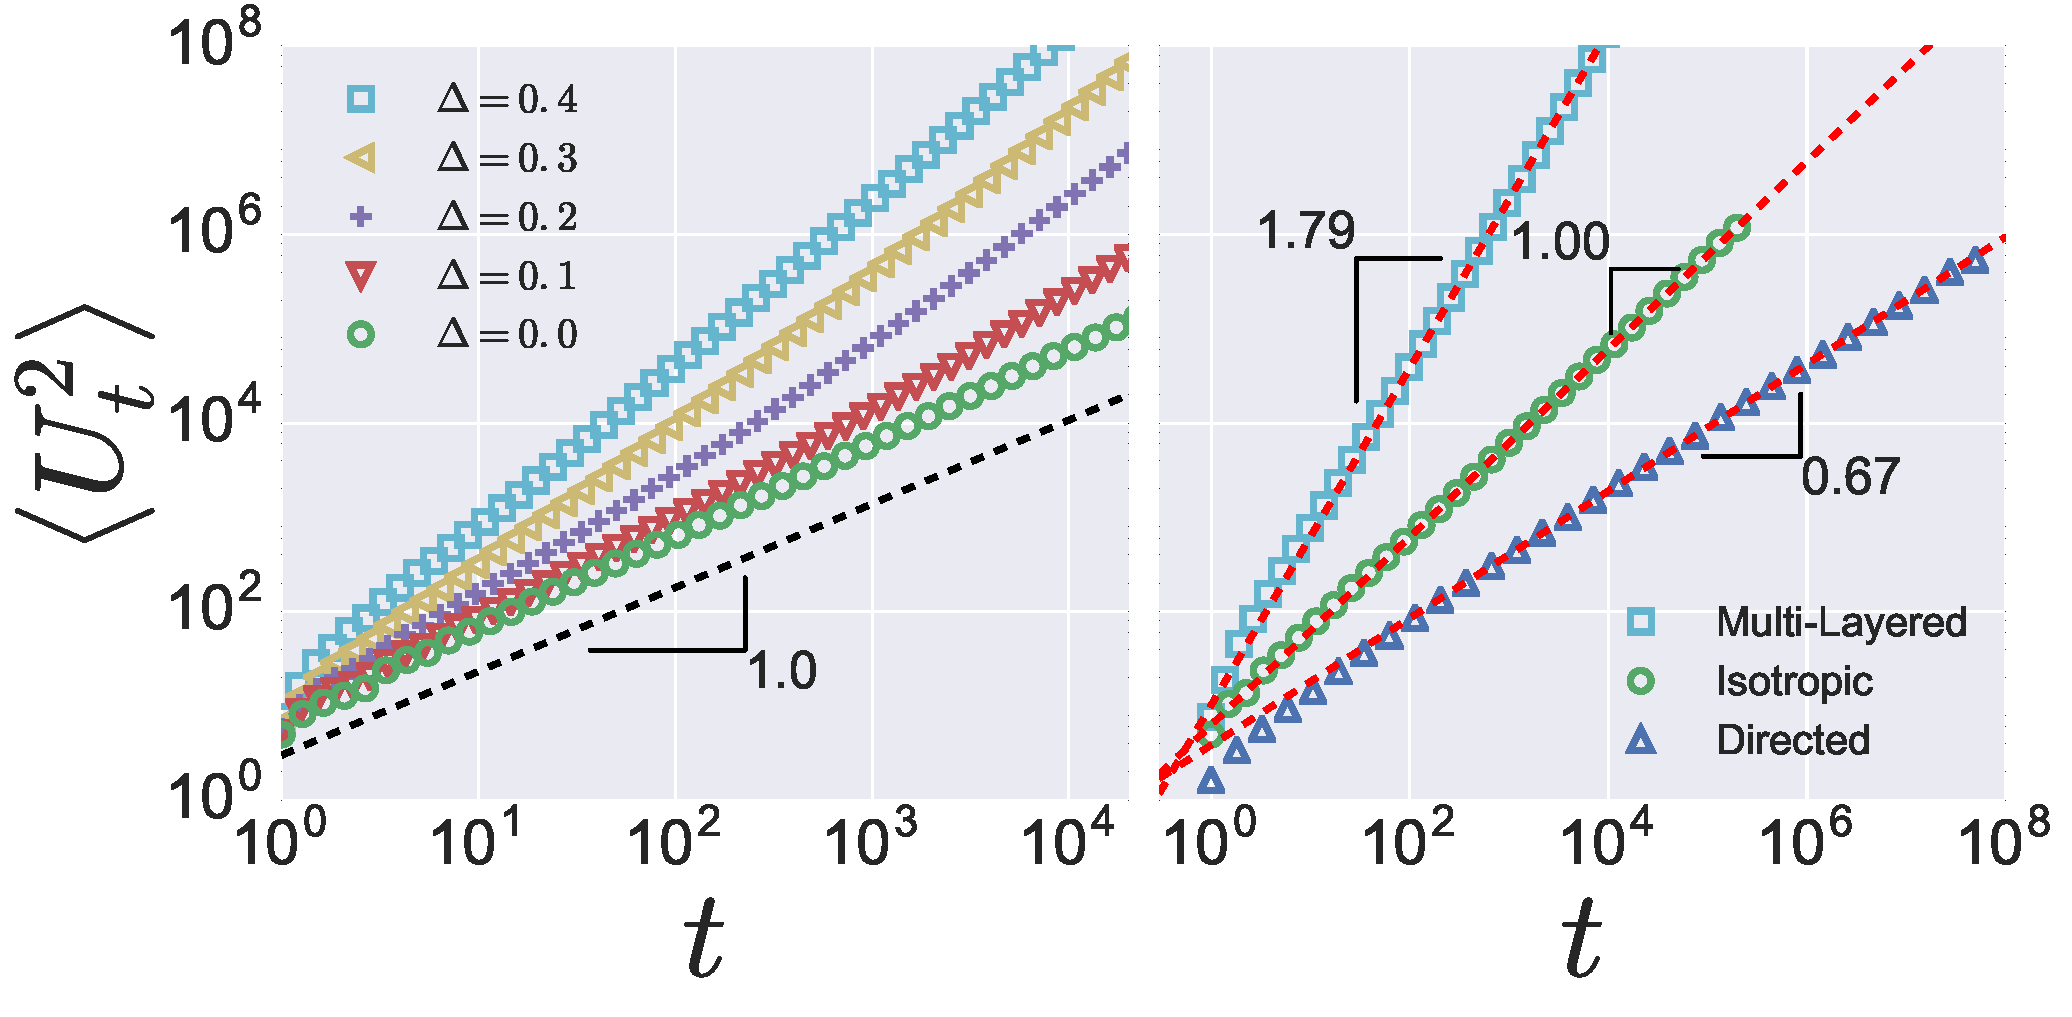
\includegraphics[width=0.8\textwidth]{chapters/ch6-asle/figs/diffusion}
\end{center}
\caption{Mean squared displacement of the driving functions for the three
    percolation models studied. The curves are the results of the numerical
    procedure described in the text applied to $10^4$ realizations of each type
    of percolation model. As expected, in the case of isotropic percolation,
    the displacement scales linearly with time, while it shows instead a
    distinctive subdiffusive behavior for directed percolation, with an
    exponent $\alpha\approx0.67$. In the case of multi-layered percolation, a
    clear superdiffusive behavior, with an exponent $\alpha\approx1.79$, can be
    observed for $\Delta=0.4$. The left graph shows this anomalous diffusion
    regime is gradually achieved as we increase the degree of anisotropy
    $\Delta$.}
\label{fig:diffusion}
\end{figure}

In the multi-layered case, the mean square displacement exhibits characteristic
superdiffusive behavior for every value of $\Delta>0$. As can be observed in
Figure~\ref{fig:diffusion}, however, a long transient behavior is present for
small values of $\Delta$ before a distinctive power-law behavior is
established. For $\Delta=0.4$, after a short transient, the fit of the data
gives a power-law with $b=10.38\pm0.68$ and $\alpha=1.78\pm0.01$, which extends
over more than three orders of magnitude. The multi-layered model is expected
to have the same continuum limit for every value of
$\Delta>0$~\cite{Dayan1991}, which should translate in driving functions with
identical exponents as $t\rightarrow\infty$ in all cases. While a qualitative
assessment of Figure~\ref{fig:diffusion} indicates that this seems to be the
case, we could not establish this hypothesis numerically as it demands
simulations of even larger traces; not possible with our current computational
power in a timely manner. 

\begin{table}[t]
\begin{centering}
\begin{tabular}{rll}
\bottomrule[0.1mm]
\toprule[0.1mm]
\textbf{Model}  & $\mathbf{b}$        & \boldmath$\alpha$   \\
\toprule[0.1mm]
Isotropic       & $6.27\,\,\,\pm0.30$ & $0.996\pm0.005$     \\[0.2cm]
Multi-Layered   & $10.38\pm0.68$      & $1.78\,\,\,\pm0.01$ \\[0.2cm]
Isotropic       & $3.74\,\,\,\pm0.07$ & $0.676\pm0.001$     \\[0.2cm]
\bottomrule[0.1mm]
\toprule[0.1mm]
\end{tabular}
\par\end{centering}
\caption{Diffusive properties of the driving function obtained from the cluster
    perimeters of each percolation model studied. In the general case the the
    mean square displacement evolves like $\left\langle U_t\right\rangle\sim
    bt^\alpha$. We observe the isotropic percolation display regular diffusion,
    as expected, while multi-layered and directed percolation are
    superdiffusive and subdiffusive respectively. The multi-layered case used
    $\Delta=0.4$.}
\label{tab:diff}
\end{table}


Again, using the same simulation setup, we tested the perimeters of the spanning
clusters of directed percolation. From the ensemble of the generated driving
functions, once more the resulting mean square displacement displays a
characteristic anomalous behavior. Precisely, the least-squares fit to the data
in the scaling region yields subdiffusive diffusion, as shown in
Figure~\ref{fig:diffusion}, with a pre-factor $b=3.74\pm0.07$ and an exponent
$\alpha=0.676\pm0.001$.

\subsection{Hurst exponents}
\label{sec:hurst}

To get a better feel of what kind of stochastic process is behind the driving
functions of our test models, we checked for the presence of long range
correlations using the detrended fluctuation analysis (DFA, see
Secion~\ref{sec:dfa}). The results are found in Figure~\ref{fig:dfaresults}. As
expected, the Brownian motion of isotropic percolation is uncorrelated, with
$H=0.5$. Multi-layered percolation shows a strongly correlated exponent of
$H=0.8$, which is consistent with the superdiffusive behavior we found. The
results of directed percolation, however, were not conclusive. The fluctuation
function does not have a power-law behavior, so a Hurst exponent cannot be
determined. This kind of anomaly can be caused by processes that are
non-stationary in non-trivial ways~\cite{Hu2001, Chen2002}. This suggests that
the driving functions of directed percolation might be of a more complicated
nature than that of isotropic and multi-layered percolation. Furthermore, we
also added the DFA of Lévy processes, since these are the only kind of
processes studied so far that are related to anisotropic scaling in SLE traces.
This kind of process however have no long range correlations, as evidenced by
the fact that $H=0.5$, so the behaviors of multi-layered and directed
percolation are not consistent with this kind of process.
\clearpage

\begin{figure}
\begin{center}
    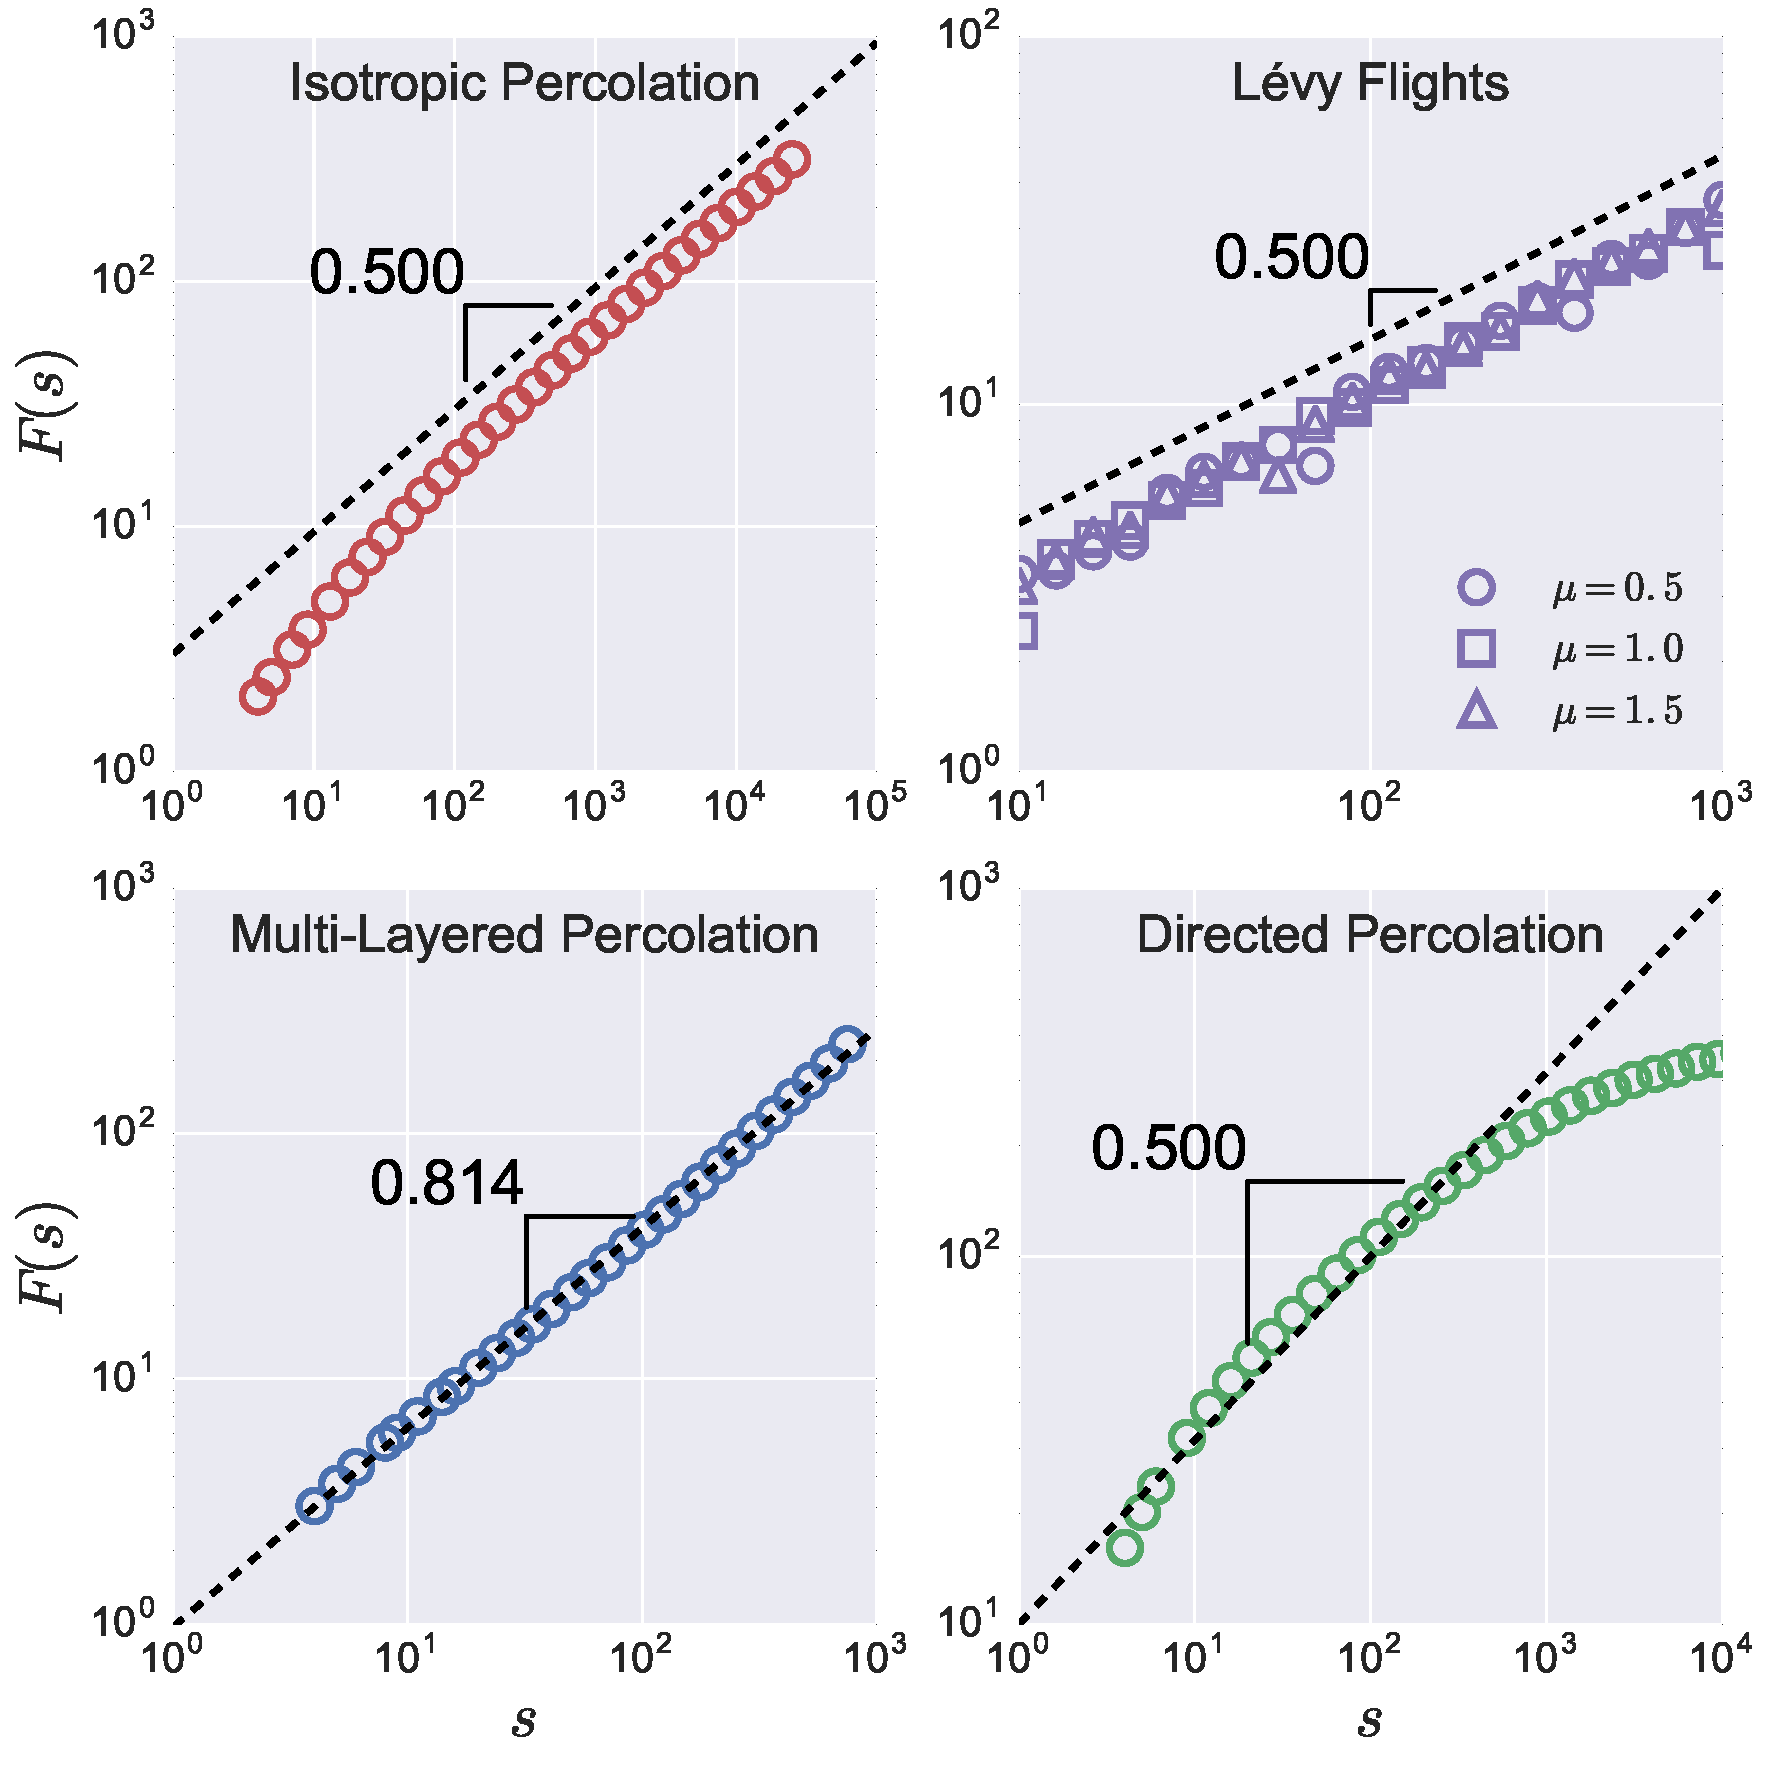
\includegraphics[scale=0.45]{chapters/ch6-asle/figs/dfaresults}
\end{center}
\caption{Results of detrended fluctuation analysis (DFA) of the driving
    functions of percolation models. As expected, the driving function of the
    isotropic percolation (top left) is a Brownian motion, therefore have
    $H=0.5$. For comparison the DFA of L\'evy flights with several $\alpha$ is
    shown (top right). Despite displaying anomalous diffusion, it still have
    $H=0.5$. Multi-layered percolation however shows a very distinct exponent
    $H=0.814$, which is consistent with the diffusion exponent shown in
    Figure~\ref{fig:diffusion}. The fluctuation function of directed
    percolation does not have a power-law behavior, which could be a result of
    non-trivial non-stationarity in the series..}
\label{fig:dfaresults}
\end{figure}
\clearpage

\subsection{SLE driven by fractional Brownian motions}
\label{sec:slebh}

The diffusion and DFA results suggest that the presence of long-range
correlations and anomalous diffusion in the driving function should lead,
through the Loewner evolution process, to the anisotropic fractal traces
observed here, and vice-versa. In order to test this hypothesis, we analyze the
behavior of traces driven by stochastic processes exhibiting both these
characteristics. We choose to use fractional Brownian time series generated
according to a given Hurst exponent $H$, which is related to the diffusion
exponent by $\alpha=2H$~\cite{Mandelbrot1968}. So the mean square displacement
evolves like
\begin{equation}
    \left\langle U_{t}^{2}\right\rangle \sim bt^{2H}.
\end{equation}
We will refer to this variant of SLE, driven by fractional Brownian motion, as
SLE$(b,H)$.

We generated the drive $U_t$ as a fractional Brownian Motion with Hurst
exponent $H$ and diffusion constant $b$ in $N$ time steps $t_i$ uniformly
spaced in the interval $[0, t_f]$. In order to simulate fractional Brownian
motions with reasonable control over the diffusive constant $b$, we used the
Davies-Harte algorithm (see Section~\ref{sec:fbm}). The $\gamma_{t_i}$ were
computed from $U_{t_i}$ using the zipper algorithm (Eq.~\ref{eq:unzip1}). We
generated three ensembles of traces, each with a different set of parameters
chosen according to the results of the diffusion and DFA analysis. Each
ensemble has a reference model. The ensemble based on isotropic percolation had
$H=0.5$ and $b=6$, as these are the theoretical values expected. The ensemble
based on multi-layered percolation used $H=0.8$ and $b=16.0$, because these
were approximately the values obtained in the previous analyses. And the direct
percolation ensemble used $H=0.33$ and $b=3.8$, based on the diffusion exponent
$\alpha=0.66$ since we could not obtain an estimate of $H$. The values of all
the parameters used can be seen in Table~\ref{tab:param}. The fractional
Brownian motions generated are much like the ones in Figure~\ref{fig:fbm} and
some examples of the resulting traces are shown in
Figure~\ref{fig:asle_traces}.

To generate traces long enough to allow for the next analyses, we relied on a
GPU (graphics processing unit) parallelized~\cite{Che2008} version of the
Zipper algorithm. The parallelization was fairly straightforward, where each
thread of execution computed a single point of the trace. We used a used a
Nvidia graphics card model Quadro K5000 with 1536 CUDA cores.

\begin{figure}
\begin{center}
    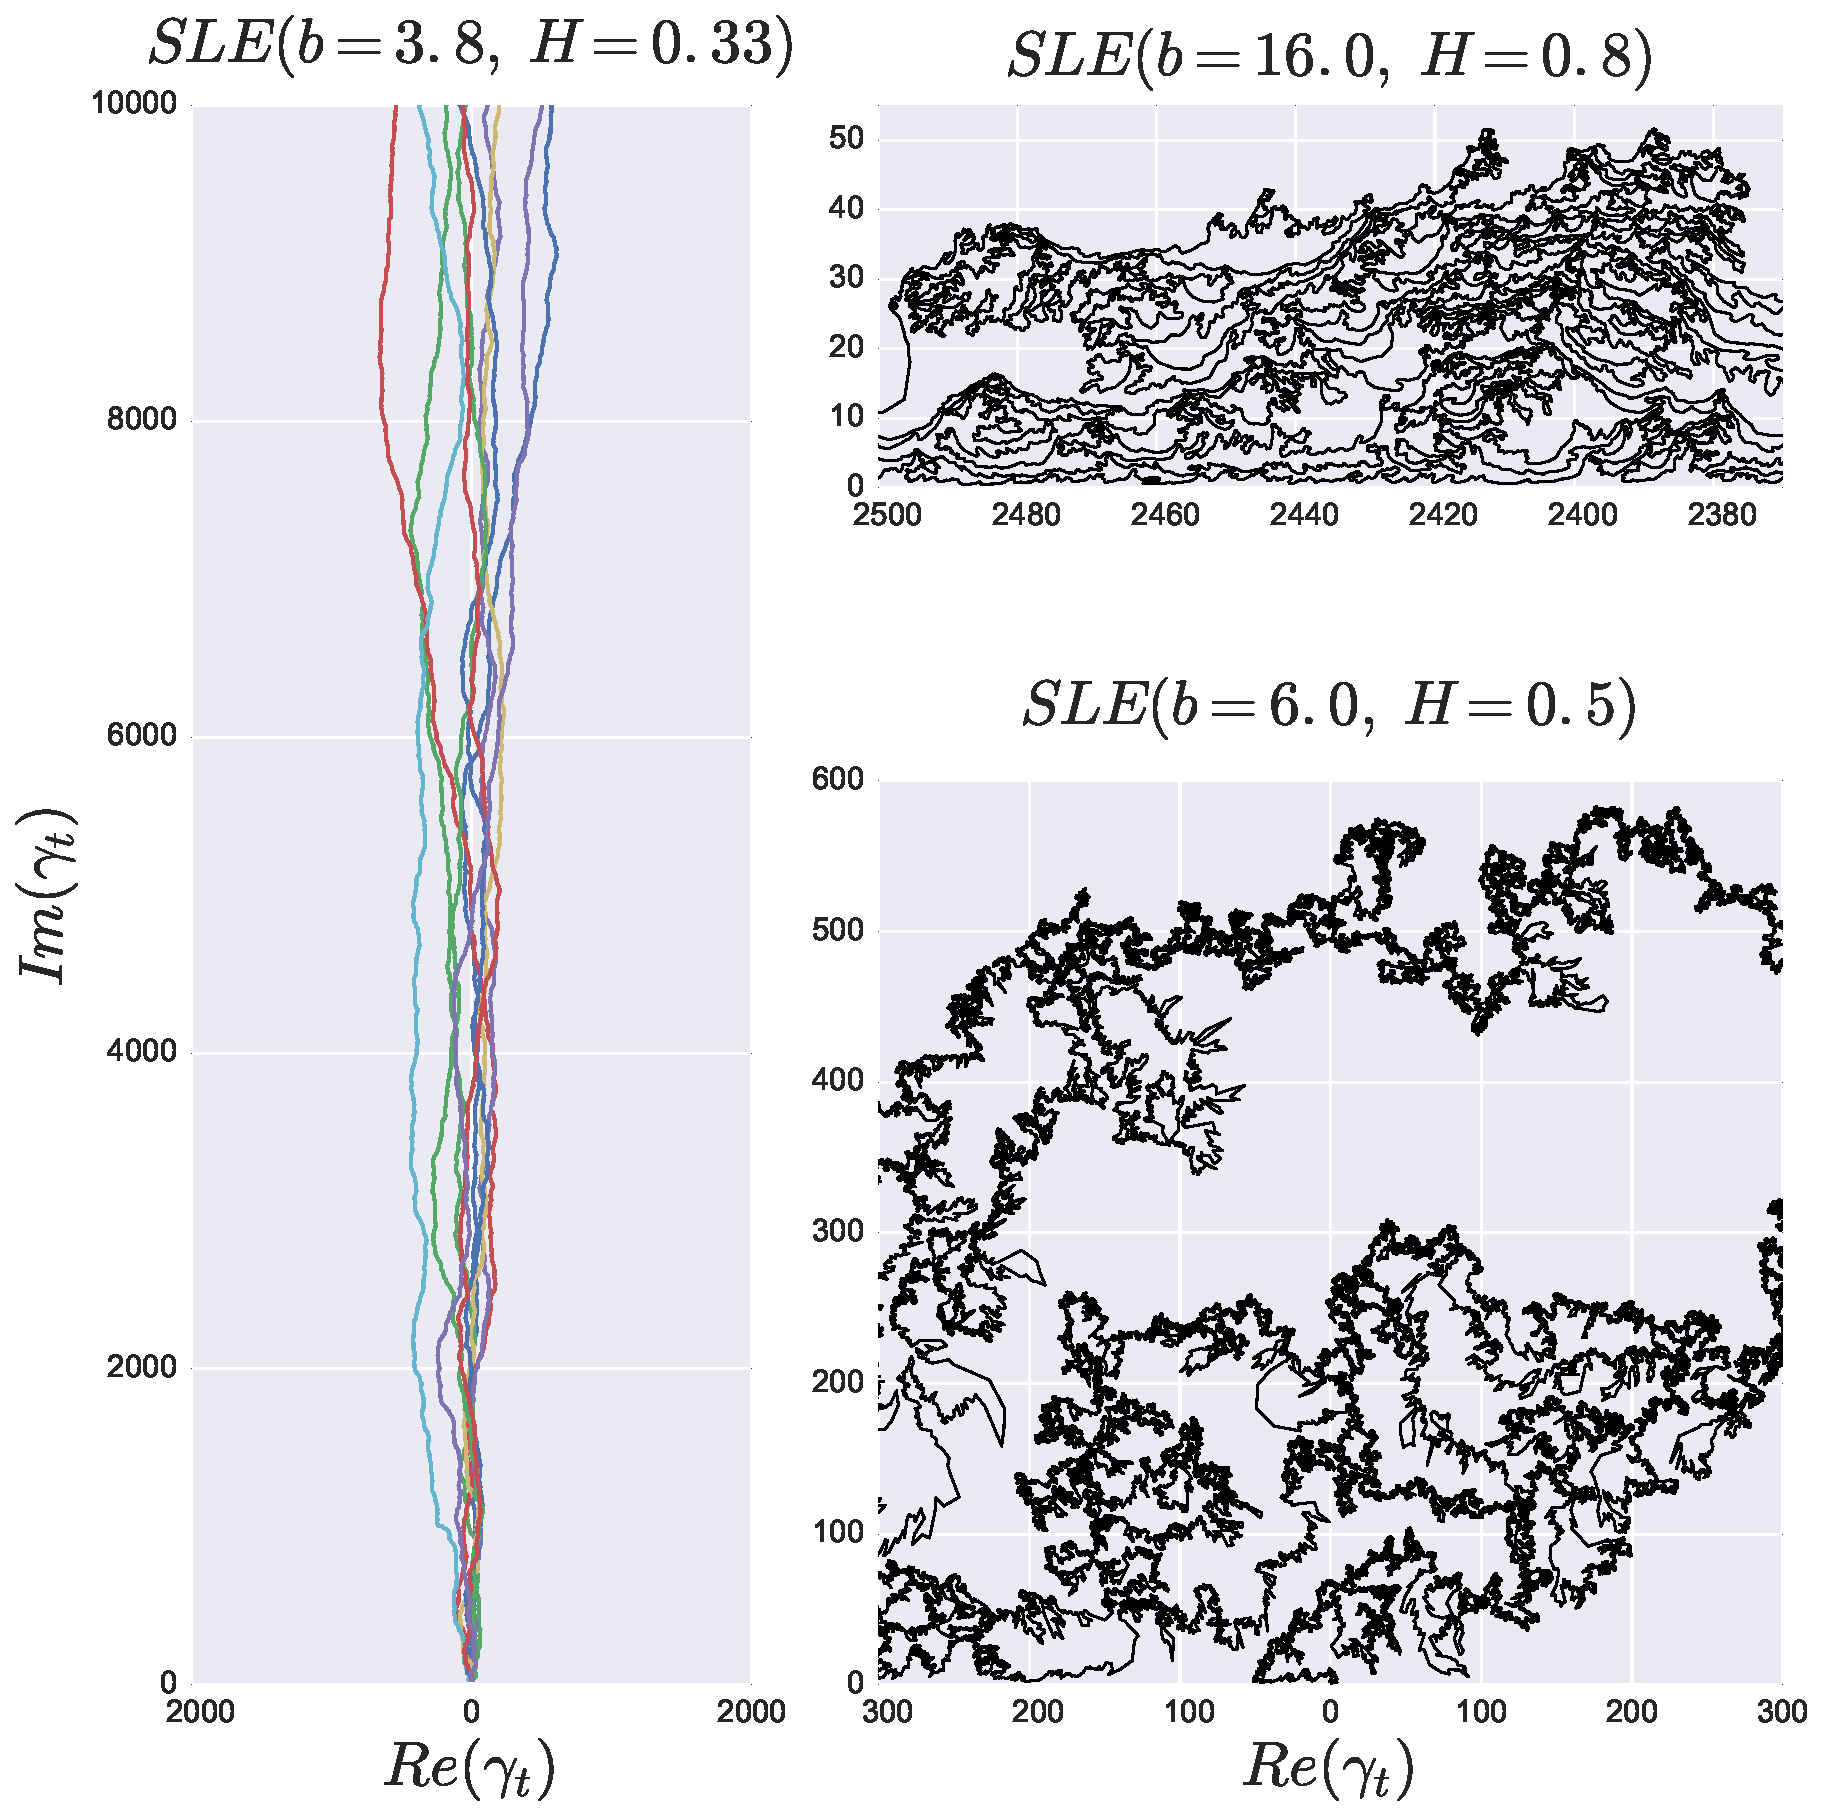
\includegraphics[scale=0.5]{chapters/ch6-asle/figs/asle_traces}
\end{center}
\caption{Examples of $SLE(b,H)$ generate using the three sets of parameters
    that we drew from the diffusion analysis (Figure~\ref{fig:diffusion}). For
    the correlated ($H>0.5$) and uncorrelated ($H=0.5$) we show one example of
    each. In the anticorrelated we show several instances. We used the zipper
    algorithm with $10^6$ points equally spaced in the interval $t\in[0, t_f]$,
    where the values of $t_f$ used can be found in Table~\ref{tab:param}.}
\label{fig:asle_traces}
\end{figure}
\clearpage



\subsection{Scaling analysis}
\label{sec:slescal}

We now set to study the scaling properties of the SLE$(b,H)$ traces and compare
with their respective reference models.

First we look at the spatial scaling, which amounts to measure the critical
exponents $\bar{\nu}_x$ and $\bar{\nu}_y$. To do that, we reparametrize the
trace as a function of its length instead of the time. This means we will have
a sequence of points $\{\gamma(\ell_i)\}$, where
\begin{equation}
    \ell_i = \sum_{j=1}^i \left|\gamma_j-\gamma_{j-1}\right|.
\end{equation}
We then interpolate the trace $\gamma(\ell)$ in $M$ equally spaced points
$\ell_i\in[0,\ell_{\max}]$. The choices of $M$ and $\ell_{\max}$ are shown in
Table~\ref{tab:param}. We then compute the the root mean squared estimation of
the displacement of the trace, that is,
\begin{equation}
    \label{eq:correl}
    F_X(i\Delta\ell) = \sqrt{\frac{1}{M-i}
    \sum_{j=0}^{M-i}{[X(\ell_{j+i}) - X(\ell_j)]}^2 },
\end{equation}
where $X(\ell) = \mbox{Re}\{\gamma(\ell)\}$.
Analogously, $F_Y(i\Delta\ell)$ is defined taking instead
$Y(\ell)=\mbox{Im}\{\gamma(\ell)\}$. These quantities should scale like
\begin{equation}
    F_{X}\left(\Delta\ell\right)\sim\Delta\ell^{\bar{\nu}_{x}},
    \,\,\,\,\,\,\,\,\,
    F_{Y}\left(\Delta\ell\right)\sim\Delta\ell^{\bar{\nu}_{y}}.
\end{equation}

\begin{figure}
\begin{center}
    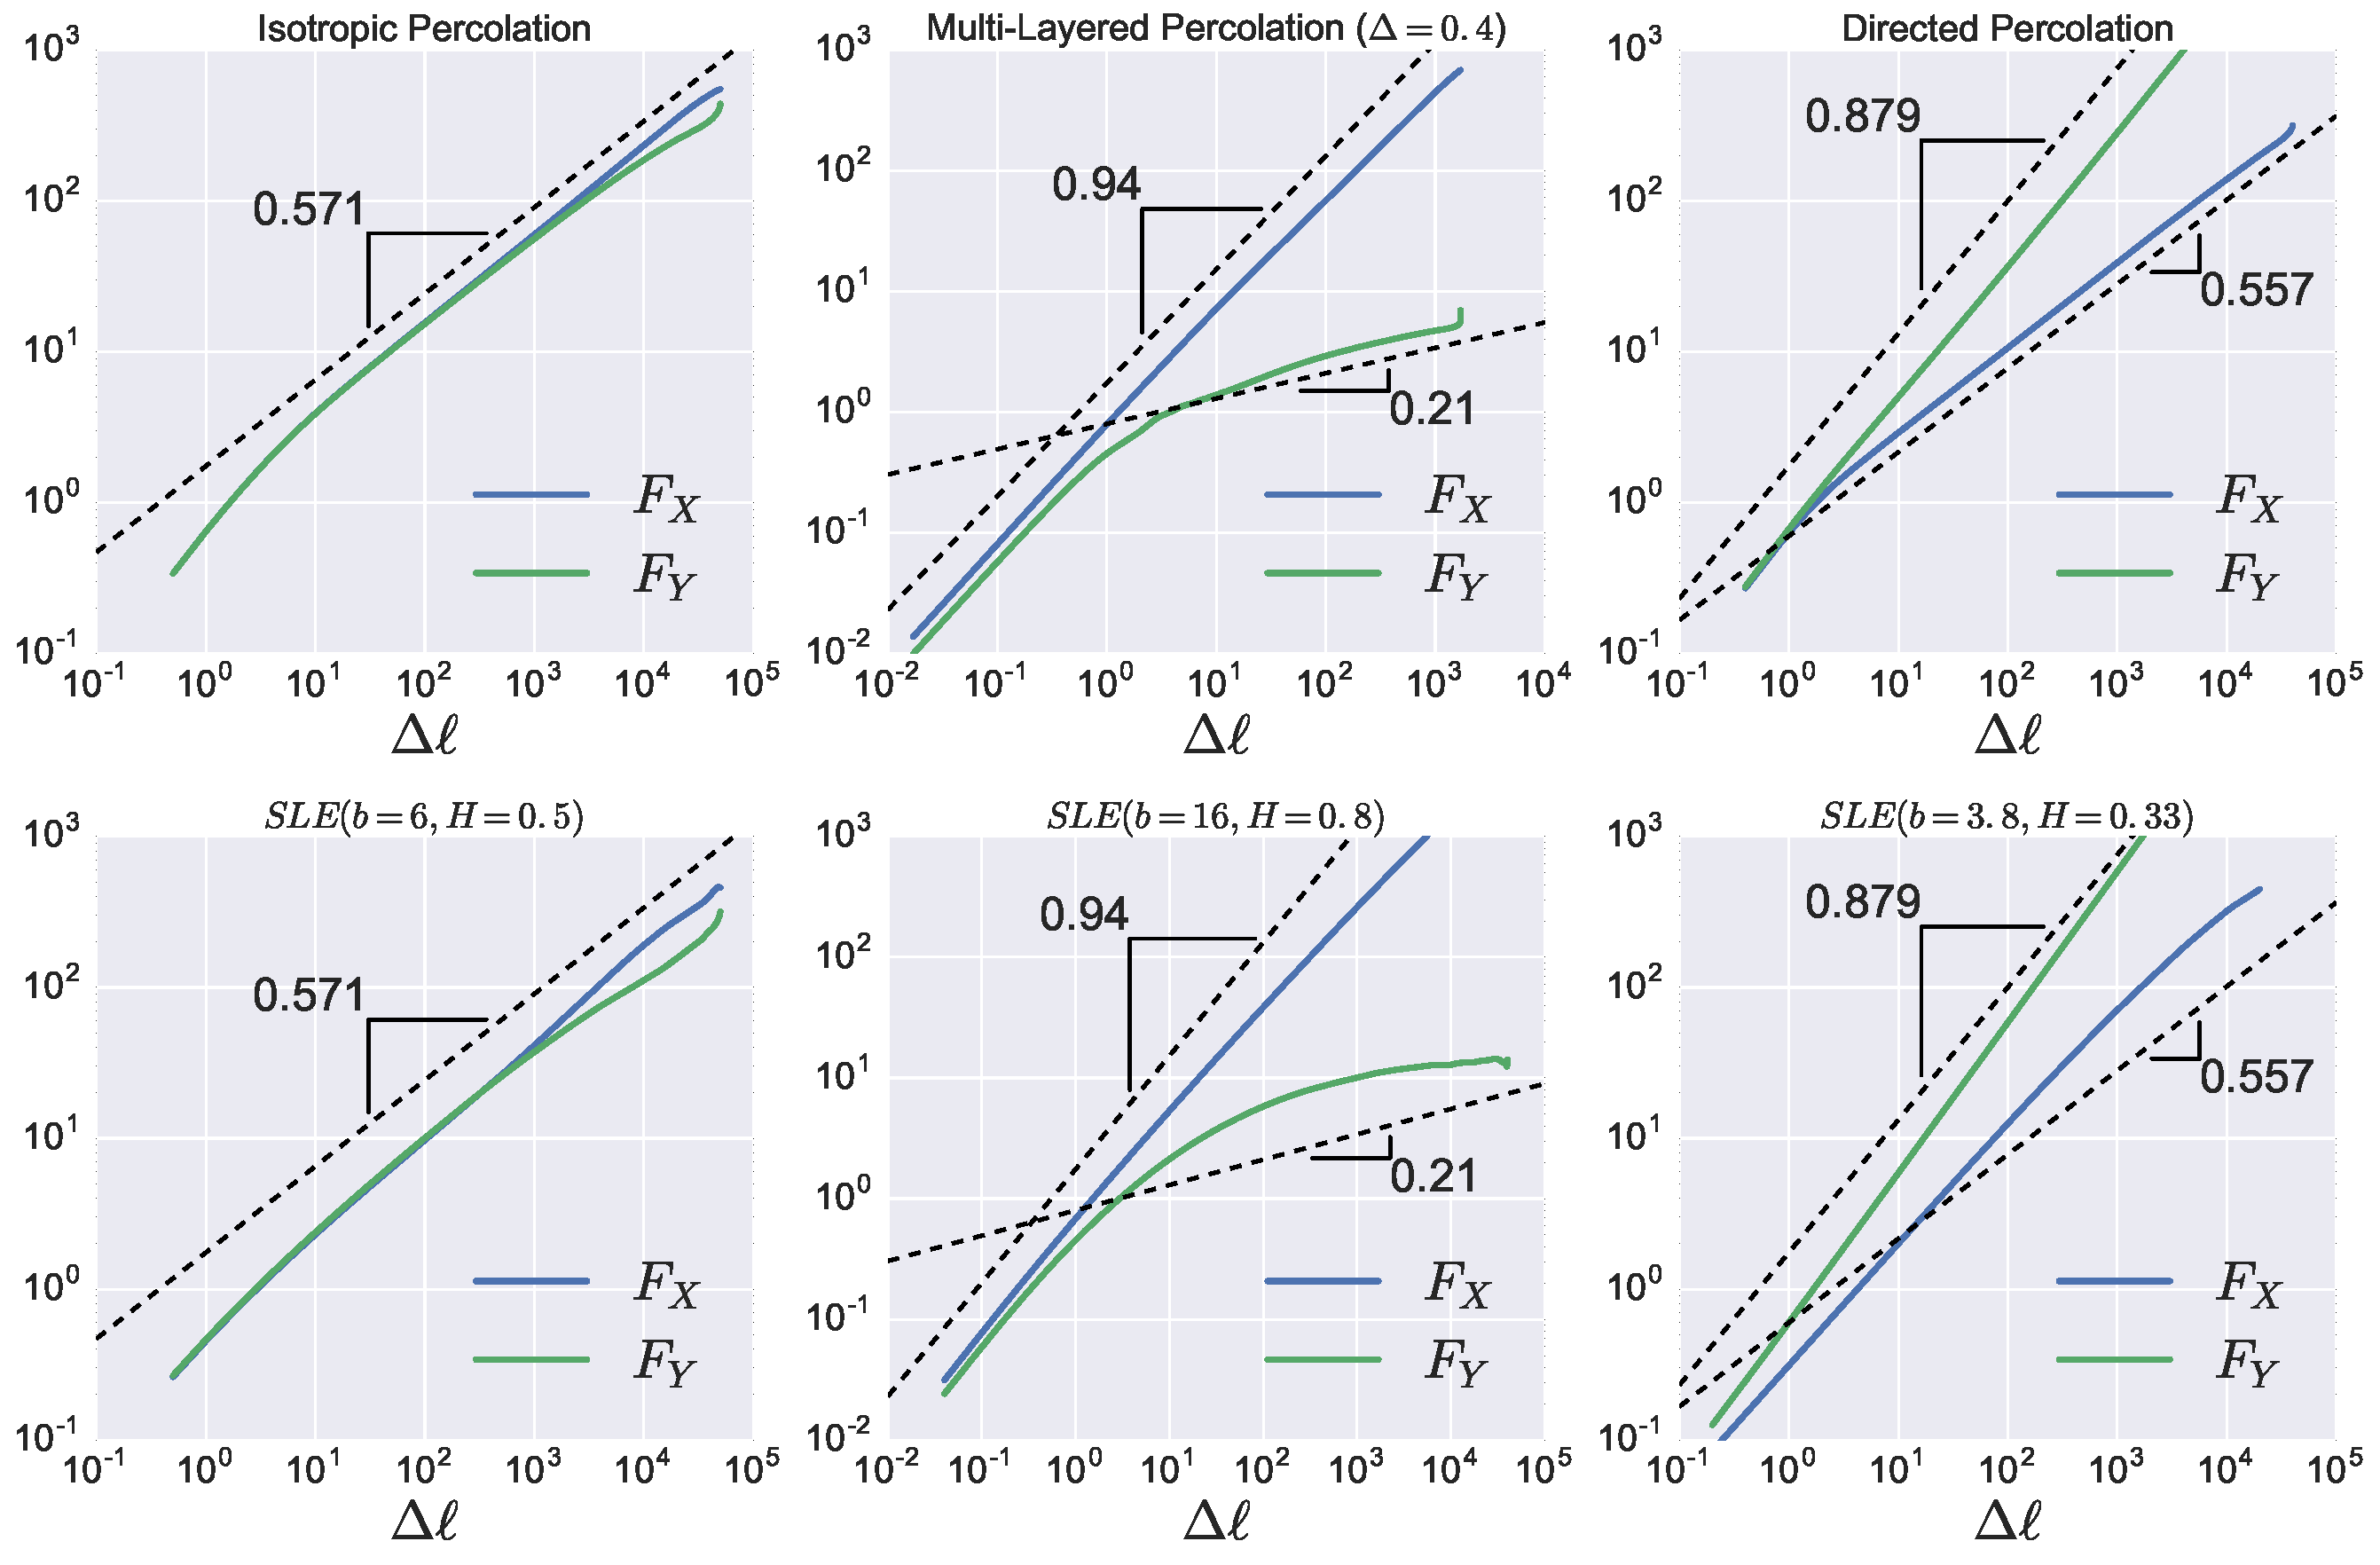
\includegraphics[width=\textwidth]{chapters/ch6-asle/figs/spacescaling}
\end{center}
\caption{Root mean squared estimations of the displacements in the X and
    Y-directions of SLE traces driven by long-range power-law correlated time
    series (fractional Brownian motion). The simulation parameters ($H$, $b$
    and $t_f$) were chosen based on the results shown in
    Fig.~\ref{fig:diffusion} (see Table~\ref{tab:param} for the numerical
    values). Good agreement is observed between the uncorrelated result
    ($H=0.5$) and isotropic percolation, as it is expected. The correlated
    trails ($H=0.8$) are also compatible with multi-layered percolation (inset
    on the bottom). In the anti-correlated case ($H=0.33$), the same kind of
    anisotropy present in the directed percolation is observed, however the
    exponents are not an exact match. These results support our hypothesis that
    long-term correlations in the driving functions, i.e., the presence of
    anomalous diffusion, are responsible for the anisotropic behavior of the
    traces. For the values of the exponents found, see Table~\ref{tab:nus}.}
\label{fig:spacescaling}
\end{figure}

\begin{figure}
\begin{center}
    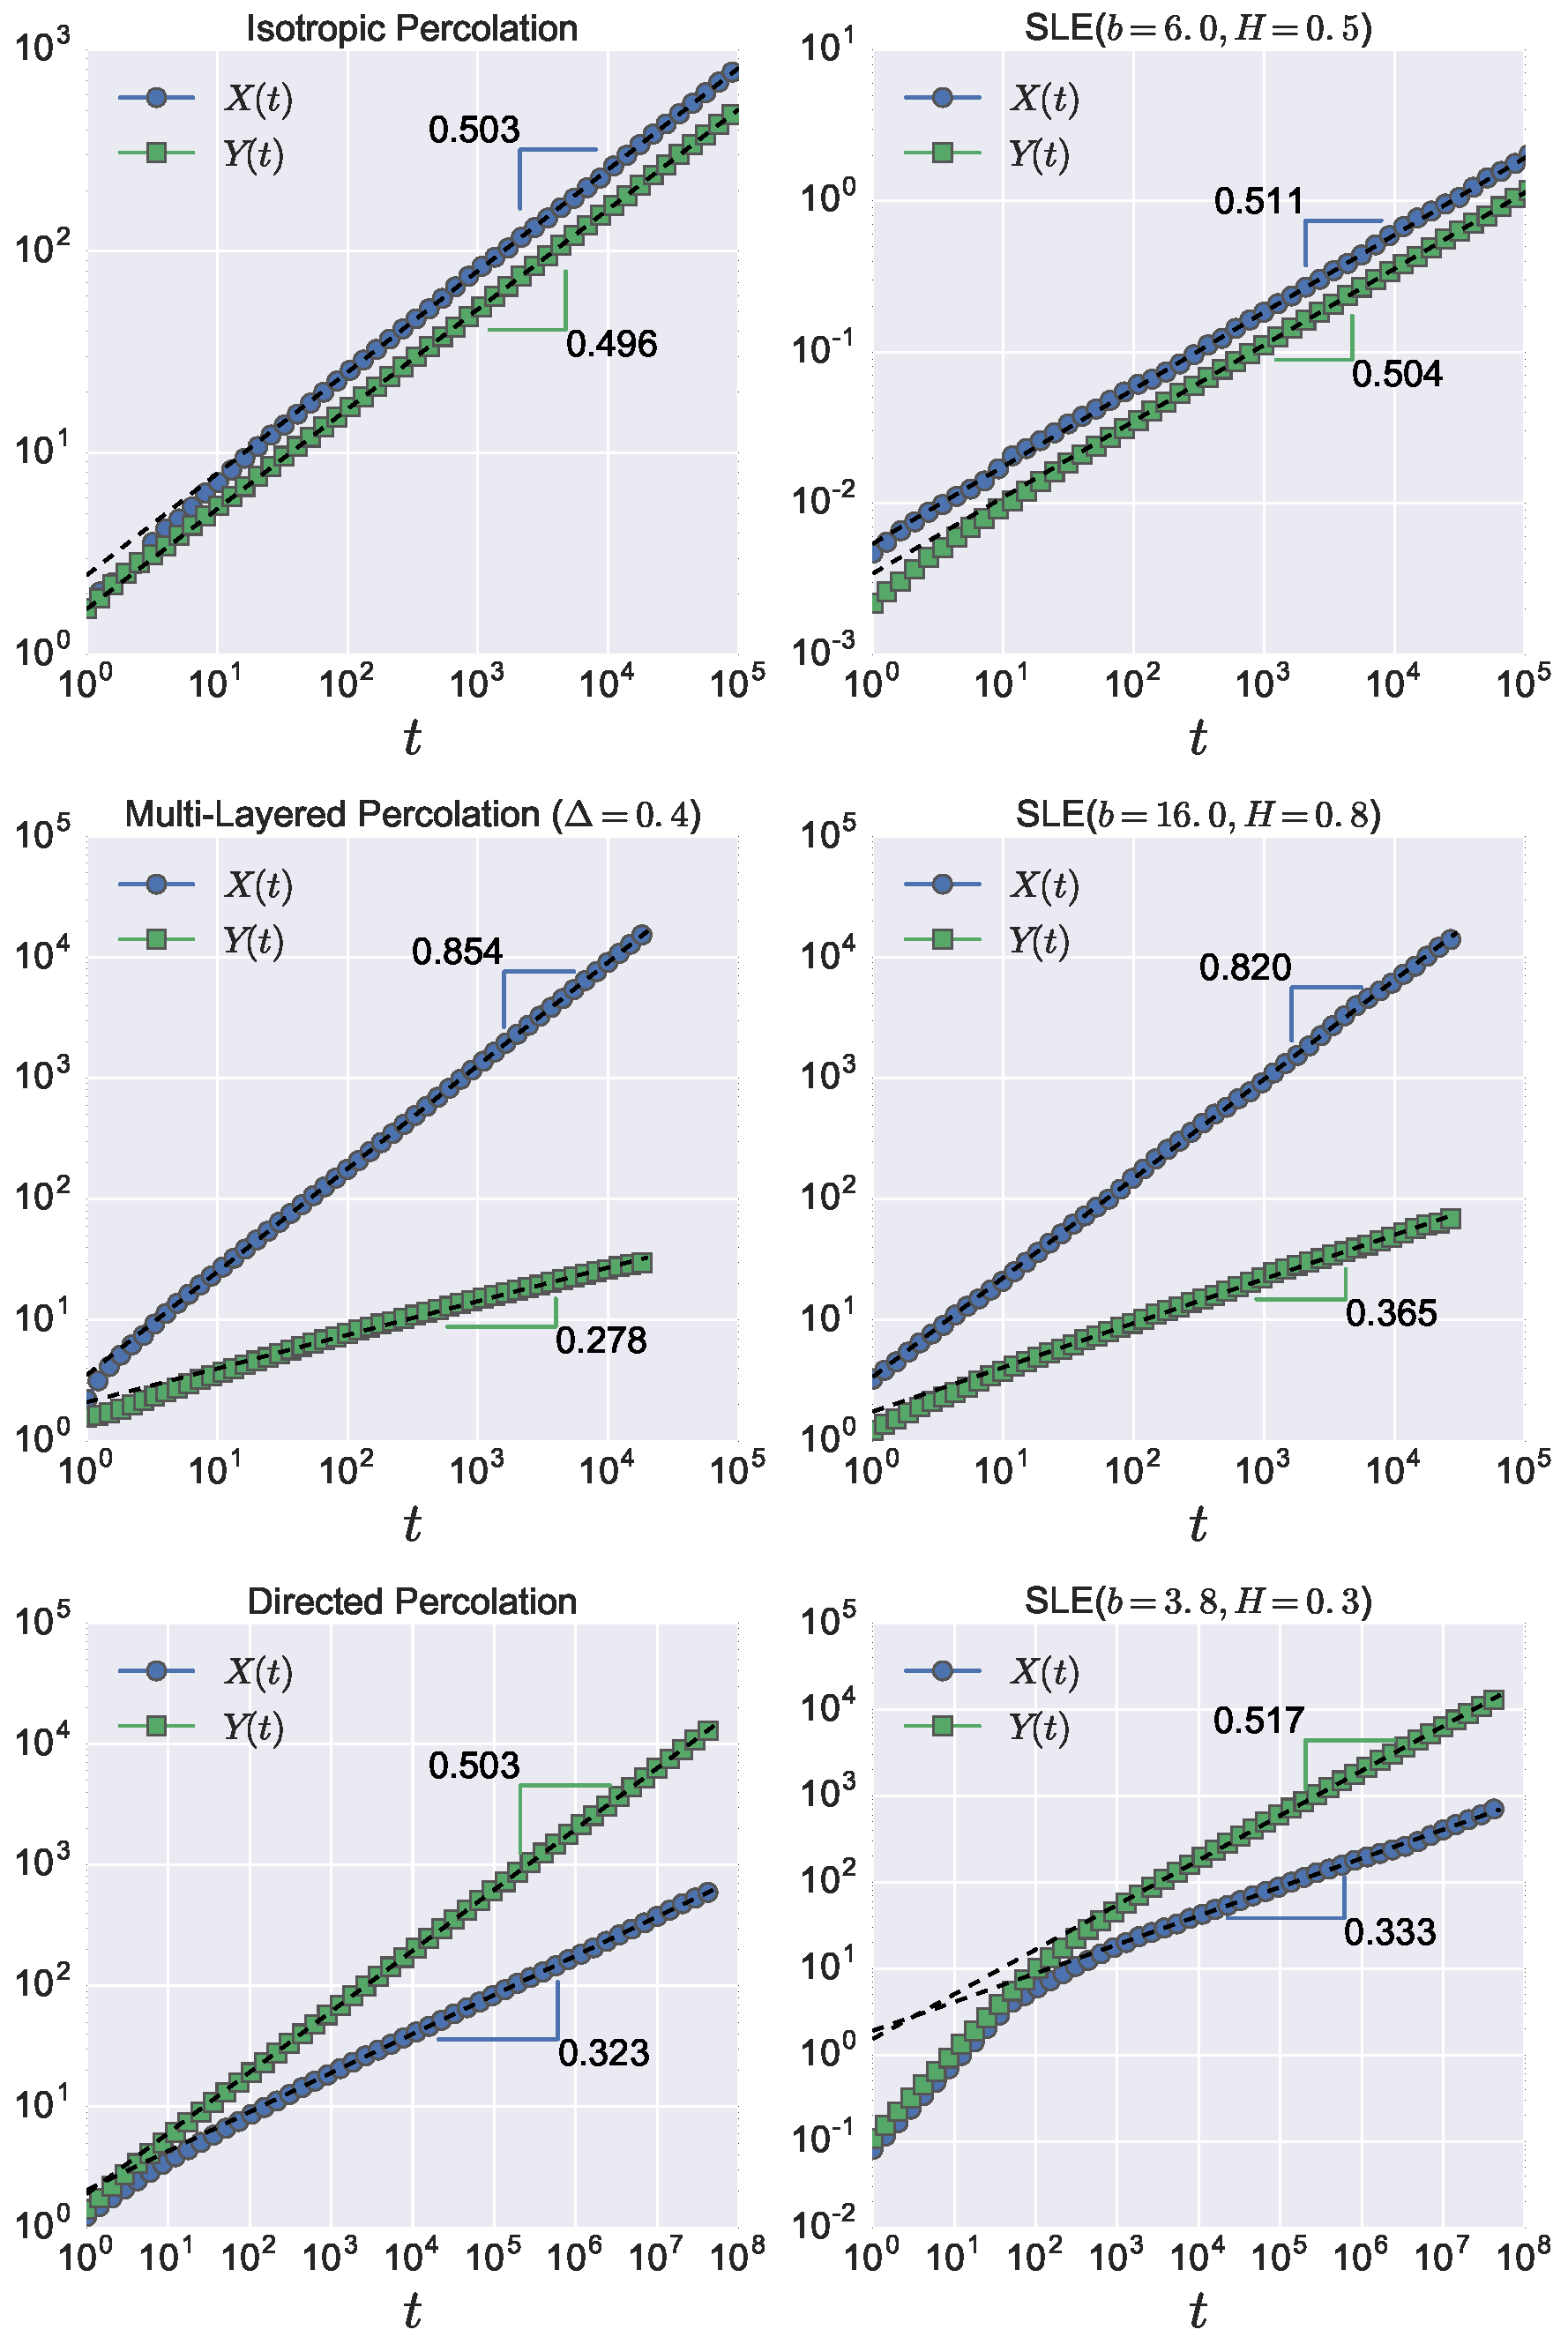
\includegraphics[width=\textwidth]{chapters/ch6-asle/figs/timescaling}
\end{center}
\caption{Scaling analysis of the percolation models and their SLE equivalents.
    Here we observe how the total width, $X(t)$, and and height, $Y(t)$, of the
    traces evolve in time. According to the SLE time.}
\label{fig:timescaling}
\end{figure}


This analysis was performed in the three ensembles of SLE$(b,H)$ traces as well
their reference models. The results are shown in Figure~\ref{fig:spacescaling}
and Table~\ref{tab:nus}. Both isotropic percolation and $SLE(6.0,\,0.5)$
yielded the expected value determined theoretically~\cite{Ziff1986}, 
\begin{equation}
    \bar{\nu}_x= \bar{\nu}_y= \frac{\nu}{1+\nu}=\frac{4}{7}\approx0.571.
\end{equation}
While the multi-layered and directed percolation exponents do not have
theoretical values, they have established numerical values in the
literature~\cite{Dayan1991, Owczarek1997}. We observed that the exponents for
the multi-layered case and the SLE$(16.0,\,0.8)$ are also coherent with one
another. However, the directed percolation case does not seems to match
$SLE(3.8,\,0.33)$. This is not completely unexpected in light of the
results we got from the DFA\@. We did however found anisotropic exponents with
the same preferential direction $\bar{\nu}_y>\bar{\nu}_x$.

\begin{table}[t]
\newcolumntype{L}[1]{>{\raggedright\let\newline\\\arraybackslash\hspace{0pt}}m{#1}}
\begin{centering}
\begin{tabular}{L{3cm}L{1.5cm}L{1.5cm}L{1.5cm}L{1.5cm}L{1.5cm}L{1.5cm}}
\bottomrule[0.1mm]
\toprule[0.1mm]
                   & $H$    & $b$    & $t_{f}$         & $N$      & $M$      & $\ell_{max}$    \\
\bottomrule[0.1mm]
Ensemble 1         & $0.5$  & $6.0$  & $2\times10^{5}$ & $10^{6}$ & $10^{5}$ & $2\times10^{4}$ \\
Ensemble 2         & $0.8$  & $16.0$ & $3\times10^{4}$ & $10^{6}$ & $10^{5}$ & $8\times10^{4}$ \\
Ensemble 3         & $0.33$ & $3.8$  & $5\times10^{7}$ & $10^{6}$ & $10^{5}$ & $2\times10^{4}$ \\
\bottomrule[0.1mm]
\toprule[0.1mm]
\end{tabular}
\end{centering}
\caption{Simulation parameters used to generate the SLE traces. $H$ is the
    Hurst exponent and $b$ is the diffusion coefficient of the fractional Brownian
    motion used as driving function. The curves were computed for $N$ times $t_i$
    equally spaced in the interval $[0, t_f]$. The resulting trace is
    reparametrized as a function of its length and interpolated in $M$ points
    equally spaced in the interval $[0,\ell_{max}]$.}
\label{tab:param}
\end{table}


\begin{table}
\begin{centering}
\begin{tabular}{rclll}
\bottomrule[0.1mm]
\toprule[0.1mm]
                                                                    &                 & \textbf{Isotropic}  & \textbf{Multi-Layered} & \textbf{Directed}   \\
\toprule[0.1mm]
\multirow{2}{*}{\textbf{Literature}}                                & $\bar{\nu}_{x}$ & $0.571$             & $0.94\,\,\,\pm0.01$    & $0.557\pm0.001$     \\[0.1cm]
                                                                    & $\bar{\nu}_{y}$ & $0.571$             & $0.21\,\,\,\pm0.01$    & $0.879\pm0.001$     \\[0.1cm]
\toprule[0.1mm]
\multirow{2}{*}{\textbf{MC Estimation}}                             & $\bar{\nu}_{x}$ & $0.573\pm0.001$     & $0.894\pm0.001$        & $0.559\pm0.004$     \\[0.1cm]
                                                                    & $\bar{\nu}_{y}$ & $0.565\pm0.001$     & $0.289\pm0.005$        & $0.898\pm0.001$     \\[0.1cm]
\toprule[0.1mm]
\multirow{2}{*}{\textbf{SLE}$\left(b,H\right)$ \textbf{Estimation}} & $\bar{\nu}_{x}$ & $0.62\,\,\,\pm0.01$ & $0.863\pm0.003$        & $0.73\,\,\,\pm0.01$ \\[0.1cm]
                                                                    & $\bar{\nu}_{y}$ & $0.55\,\,\,\pm0.01$ & $0.21\,\,\,\pm0.01$    & $1.000\pm0.001$     \\[0.1cm]
\bottomrule[0.1mm]
\toprule[0.1mm]
\end{tabular}
\par\end{centering}
\caption{Critical exponents $\bar{\nu}_x$ and $\bar{\nu}_y$ relative to the
    spatial scaling of the cluster perimeters in the three percolation models
    studied here. Literature values were taken from~\cite{Ziff1986, Dayan1991,
    Owczarek1997}. Isotropic percolation is the only one for which the
    exact value is know, $\bar{\nu}_x= \bar{\nu}_y= 4/7\approx0.571$. We
    estimated the exponents of each model using Monte Carlos methods, by
    generating cluster perimeters and using Eq.~\ref{eq:correl}. We also estimated the
    exponents of their possible SLE$(b,H)$ (using the parameters given in
    Table~\ref{tab:param}). There's reasonable accordance between the exponents
    of multi-layered and isotropic percolation, considering the limitations of
    the method. Directed percolation, however, is not a match, suggesting that
    it may not be described by a SLE$(b,H)$.}
\label{tab:nus}
\end{table}


We also looked at how the traces scale with the SLE time. To do this we looked
at the characteristic length scales of the traces, $X(t)$ and $Y(t)$,
equivalent to the width and height of the hull at time $t$. Much like with the
spatial scaling, we compared the percolation models and their equivalent
SLE$(b,H)$. The results are shown in Figure~\ref{fig:timescaling}. The
isotropic percolation and SLE$(6.0,\, 0.5)$ both have $X\approx Y~t^{0.5}$, is
in accordance with Eq.~\ref{eq:aniscale} with $\mu=2$, again as expected. The
multi-layered case is also behaves very similarly with the SLE$(16.0,\,0.8)$.
Now, somewhat surprisingly, the directed percolation result seems to match
pretty closely the SLE$(3.8, 0.33)$ exponents, with $X~t^{0.33}$ and
$Y~t^{0.5}$ approximately. It is unclear why this particular test showed
similar exponents, while the spatial scaling did not. One possibility is that
the temporal scaling of the traces is more influenced by the diffusive
properties of the drive than by the presence of long range correlations.


\chapter{Conclusion}
\label{sec:concl}

So we reach the end of this work. We hope that by now we made clear the
importance and impact that the study of critical systems has had in both
physics and mathematics. In our research we took to ourselves to explore two
little understood areas: strongly anisotropic systems and Schramm-Loewner
evolutions driven by non-Brownian stochastic processes.

Strong anisotropy is the observed property that some systems have where several
quantities behave differently depending on which direction you are measuring
them. Particularly, we looked at two variants of the percolation model that
display anisotropy. The first, Multi-layered percolation, was designed to
simulate the transport properties in stratified (layered) media. The second,
directed percolation, mimics the filtering of a fluid along a porous medium
under the effect of gravity, so it flows only along a predetermined direction.

We generated an ensemble of cluster perimeters in isotropic, multi-layered, and
directed percolation, then used the zipper algorithm to compute the driving
function from these curves and, looking at their diffusive properties, we found
that they are anomalously diffusive. Multi-layered percolation is associated
with superdiffusive driving functions while directed percolation with
subdiffusive ones. This is the first time a physical model has been associated
to driving functions with these properties.

Furthermore, a detrended fluctuation analysis of the driving functions yielded
mixed results. Multi-layered percolation showed a discernible positive
correlation with a Hurst exponent $H\approx0.8$. Directed percolation however
had inconclusive results, where the fluctuation function did not behave as a
power law, as it would be expected. This could happen because of irregular
behaviors in the series, like non-stationarity or the presence of
singularities.

In the second part of this work, we went one step further and looked at the
opposite procedure, that is, what kind of traces we would obtain if we used
anomalously diffusive processes as driving functions. We chose to use
fractional Brownian motions with the parameters obtained from the previous
analysis. We found that the resulting traces have a scaling behavior consistent
with the multi-layered percolation. For directed percolation, again results
were mixed. While the traces do not have spatial scaling exponents consistent
with lattice model, the scaling in SLE time was surprisingly close.

In summary, our numerical analysis offers compelling evidence that a variation
of the Stochastic Loewner Evolution, obtained by taking as driving function a
stochastic process with anomalous diffusion, may be the scaling limit of
anisotropic critical models. In particular, multi-layered percolation seems to
have as scaling limit an SLE driven by a fractional Brownian motion with hurst
exponent $H\approx0.8$ and diffusive constant $b\approx16$. The same could not
be asserted for the directed percolation case, indicating that there is more to
strong anisotropy than simply anomalous diffusion. We expect that the further
developments of this new variant of SLE may provide some insight on the
critical behavior of anisotropic systems, the same way the original SLE was to
isotropic systems.
